\documentclass[nativefonts,print]{Style/class_dissertation}


%%%%%%%%%%%%%%%%%%%%%%%%%%%%%%%%%%%%%%%%%%%%%%%%%%%%%%%%%%%%%%%%%%
% Stuff added by MW
%\newcommand{\red}[1]{\textcolor{red}{#1}}
	% This can be found in the PackagesNewCommands directory+file
%%%%%%%%%%%%%%%%%%%%%%%%%%%%%%%%%%%%%%%%%%%%%%%%%%%%%%%%%%%%%%%%%%

% load a collection of convenient shortcut commands


% Written by Noreen Walker,
% see also Thesis\Commands\additional_custom_commands
% For additional code by MW


% Define new convenient shortcut commands and include packages

% *******************************************
% include extrapackages
% *******************************************
\usepackage{soul}				% yellow highlighting \hl{}
\usepackage{textgreek}			%greek upright letters in text mode
\usepackage{xifthen}			%if statements, optional arguments in newcommand
\usepackage[export]{adjustbox}  %align images withing figure environment (left,right)
%\usepackage{endnotes}			%doesn't really work
\usepackage{placeins}			% prevent floats from floating behind the chapter end 	
%\usepackage{booktabs}			% nicer tables
\usepackage{tabu}				% thick lines in tables
\usepackage{colortbl}			% colored cells in tables
\usepackage{bm}					% bold math symbols
\usepackage{mdwlist}			% compact (itemize) lists: itemize*
\usepackage{float}				% enforce float-figure position, e.g. [H]
\usepackage{xfrac}				% small (inline) fractions (\sfrac)

% *******************************************
% Layout
% *******************************************
\renewcommand{\footnotesize}{\small}	% change footnotesize (increase to "small")
\newcommand{\defaultlinesep}{\tabulinesep = 0.8mm} % define a height separation for tables (tabu package)
\newcommand{\cellgray}{\cellcolor[rgb]{0.85 0.85 0.85}} % background color in tables
\newcommand{\cellbright}{\cellcolor[rgb]{0.92 0.92 0.92}} % background color in tables



% *******************************************
% Correction
% *******************************************
% red text
\newcommand{\red}[1]{\textcolor{red}{#1}}
% red text in brackets
\newcommand{\bred}[1]{\textcolor{red}{(#1)}}
% red text with "ToDo:"
\newcommand{\todo}[1]{\textcolor{red}{ToDo: #1}}
% red text
\newcommand{\blue}[1]{\textcolor{blue}{#1}}
% shortcut for underlining text and red
%\newcommand{\e}[1]{\textcolor{red}{#1}} % DISABLED TO MAKE TEXT BLACK AGAIN
\newcommand{\e}[1]{{#1}}
\newcommand{\ee}[1]{{#1}}
%\newcommand{\ee}[1]{\textcolor{red}{#1}}
% missing reference. set argument to empty if ref. not known
\newcommand{\missref}[1]{\ifthenelse{\equal{#1}{}}{\hl{[ref?]}}{\hl{[ref: #1 ]}}}

% Alternative: \missref and \missref[text]
%\newcommand{\missref}[1][]{%
%	\ifthenelse{\equal{#1}{}}{\hl{[ref?]}}{\hl{[ref: #1 ]}}%
%	}



% *******************************************
% Frequently used expression
% *******************************************
% Ecoli
\newcommand{\ecoli}{\textit{E. coli }}
% Delta cAMP
\newcommand{\dcamp}{$\Delta$cAMP }
% P_lac
\newcommand{\plac}{\ensuremath{\text{P}_{\text{lac}}\text{ }}}
% P_N25
\newcommand{\pntwofive}{\ensuremath{\text{P}_{\text{N25}}\text{ }}}
% P_lambda
\newcommand{\plambda}{\ensuremath{\text{P}_{\lambda}\text{ }}}
% P_rrn
\newcommand{\prrn}{\ensuremath{\text{P}_{\text{rrn}}\text{ }}}
% P_rrn-GFP
\newcommand{\prrnGFP}{\ensuremath{\text{P}_{\text{rrn}}\text{-GFP }}}
% lac in italics
\newcommand{\lac}{\textit{lac }}
% crosscorr: R_pmu(tau) 
\newcommand{\Rpmut}{\ensuremath{R_{p\mu}(\tau)} }
% crosscorr: R_pmu
\newcommand{\Rpmu}{\ensuremath{R_{p\mu}} }
% crosscorr: R_Emu(tau) 
\newcommand{\REmut}{\ensuremath{R_{E\mu}(\tau)} }
% crosscorr: R_Emu
\newcommand{\REmu}{\ensuremath{R_{E\mu}} }
% . [point] with hspace before (for equations)
\newcommand{\spacepoint}{\hspace{5px} .}
% , [comma] with hspace before (for equations)
\newcommand{\spacecomma}{\hspace{5px} ,}
 

% (A) etc for subfigures
\newcommand{\figA}{(\textbf{A}) }
\newcommand{\figB}{(\textbf{B}) }
\newcommand{\figC}{(\textbf{C}) }
\newcommand{\figD}{(\textbf{D}) }
\newcommand{\figE}{(\textbf{E}) }
\newcommand{\figF}{(\textbf{F}) }
\newcommand{\figG}{(\textbf{G}) }
\newcommand{\figH}{(\textbf{H}) }
\newcommand{\figI}{(\textbf{I}) }
\newcommand{\figJ}{(\textbf{J}) }

% --------
% Chapter6: Growth Noise
% --------
% short cut for "Extended Data" -> leaves option to change this section name/reference later on
\newcommand{\ED}{Extended Data }
\renewcommand{\NG}{\ensuremath{N_G} } % noise sources in model [this specific command already existsed for some symbol]
\newcommand{\NE}{\ensuremath{N_E} }
\newcommand{\Nmu}{\ensuremath{N_{\mu}} }
\newcommand{\NX}{\ensuremath{N_X} }
\newcommand{\TEE}{\ensuremath{T_{EE}} }	% transmission coefficients in model
\newcommand{\TmuE}{\ensuremath{T_{\mu E}} }
\newcommand{\TEmu}{\ensuremath{T_{E\mu}} }
\newcommand{\TEG}{\ensuremath{T_{EG}} }
\newcommand{\TmuG}{\ensuremath{T_{\mu G}} }


% --------
% Chapter4: Extrinsic Noise
% --------
% corr: R(Y,mu)
\newcommand{\corrYmu}{\ensuremath{R(Y,\mu)} }
% corr: R(C,mu)
\newcommand{\corrCmu}{\ensuremath{R(C,\mu)} }
% corr: R(Y,C)
\newcommand{\corrYC}{\ensuremath{R(Y,C)} }
% noise: n(Y)^2 (maybe modify to underscript Y or brackets, or even P)
\newcommand{\noiseY}{\ensuremath{\eta_Y^2} }
% noise: n(C)^2 (maybe modify to underscript C or brackets, or even P)
\newcommand{\noiseC}{\ensuremath{\eta_C^2} }
% noise: n(mu)^2 (maybe modify to underscript mu or brackets)
\newcommand{\noisemu}{\ensuremath{\eta_{\mu}^2} }
% <mu>
\newcommand{\mumean}{\ensuremath{\langle \mu \rangle} }
% standard deviation: sigma_Y (could still be modified to sigma(Y))
\newcommand{\sigmaY}{\ensuremath{\sigma_Y} }
% standard deviation: sigma_C (could still be modified to sigma(C))
\newcommand{\sigmaC}{\ensuremath{\sigma_C} }
% standard deviation: sigma_mu (could still be modified to sigma(mu))
\newcommand{\sigmamu}{\ensuremath{\sigma_{\mu}} }
% extrinsic noise (squared)
\newcommand{\noiseextr}{\ensuremath{\eta_{extr}^{2}} }
% intrinsic noise (squared)
\newcommand{\noiseintr}{\ensuremath{\eta_{intr}^{2}} }
% noise n(E)^2 (general expression noise -> meybe use Y directly)
\newcommand{\noiseE}{\ensuremath{\eta_{E}^{2}} }
% global noise intensity <N_G^2>
\newcommand{\VarNG}{\ensuremath{\langle N_G^2\rangle} } 
% protein specific noise intensity <N_P^2>
\newcommand{\VarNP}{\ensuremath{\langle N_P^2\rangle} } 
% mu in covariance decomposition (allows to switch between mu and mu^H)
\newcommand{\mucond}{\ensuremath{\mu}}%{\ensuremath{\mu^H}}
% F_extr,E (extrinsic explained fraction) (the E could be removed)
\newcommand{\Fextr}{\ensuremath{F_{extr,E}} }
% Expression noise - vs - Growth
\newcommand{\noiseEvsMu}{\ensuremath{\eta_{E}^2 \text{ vs. }\mu} } % include packages 
							 %      and define commands
							 % also additional commands are defined in Commands/additional_custom_commands, see below

% My aditions:

% To be able to print citations (doesn't seem to work in combination with hyperref according to google?)
%\usepackage{bibentry}
%\nobibliography* % needed to create a dummy bibliography apparently

%\usepackage{enumitem } % for lists w/o spacing.
\usepackage{blindtext} 
% more list options
%\usepackage[inline]{enumitem}
\usepackage{xcolor}
\usepackage{paralist}

\usepackage{upgreek} % for the upright µ symbol

\usepackage{verbatim}
\usepackage{breakurl} % in combination with sloppy and fussy commands this should allow breackage of urls, but it didn't; also \url will produce links
\usepackage{hyperref}

% In case the "d" in dx is desired to have a special markup.
\usepackage{amsmath} % also required for align environment
%\newcommand*\diff{\mathop{}\!\mathrm{d}}

% Some attempts to corretly break urls (and e.g. also script names).
% \PassOptionsToPackage{hyphens}{url}\usepackage{hyperref}
% \g@addto@macro{\UrlBreaks}{\UrlOrds}
% Suggestions from: https://tex.stackexchange.com/questions/3033/forcing-linebreaks-in-url

% \usepackage{siunitx} % e.g. \micro % does not work..

% set path for figures % TODO some thing from Noreen setting the figure path..
%% set path for figures

% 1) relative path (portable version)
% 2) dropbox folder link on Amolf computer
% 3) dropbox folder link on personal laptop (=same folder as 2)
\graphicspath{{./Figures/} {C:/Users/walker/Dropbox/PhDThesis_Figures/}  {C:/Users/Nocka/Dropbox/PhDThesis_Figures/} }


%\usepackage{graphicx} % should also enable eps??

%\usepackage{array}

% Needed for floating caption
\usepackage{graphicx} 
\usepackage{caption}

% Needed to use svg graphics
%\usepackage{svg} % does not seem to work --> use pdfs.

% Needed for eps??
\usepackage{epstopdf}

% for degree symbol
\usepackage{gensymb}

% To enable floatbarriers
\usepackage{placeins}

% misc
\usepackage{tabularx}
\usepackage{setspace}
% \usepackage{longtable} % not sure this combines with tabularx

% needed for list item separation
\usepackage{enumitem}

% hopefully to support dutch hyphenation correctly
\usepackage[dutch,english]{babel}

% For hyphenation of words that already contain a hyphen
\usepackage[shortcuts]{extdash} % Use Example\=/McExampleface to introduce "uncounted" hyphen

% Just for printing the lengths of latex variables (such as margins)
% Only needed for editing, package not needed otherwise
\usepackage{printlen}
%% The size of the text is:
%\the\textwidth
%% 362.77263pt
%\uselengthunit{cm}\printlength{\textwidth}
%% 12.74818 cm
%\uselengthunit{cm}\printlength{\textheight}
%% 19.19734 cm

% To align images to the right
\usepackage[export]{adjustbox}

% .tif images cannot be read, but we can automatically have them converted
% (This also needs \usepackage{epstopdf})
%\epstopdfDeclareGraphicsRule{.tif}{png}{.png}{convert #1 \OutputFile}
%\AppendGraphicsExtensions{.tif}
    % Unfortunately this code from the internet didn't work 
    % https://tex.stackexchange.com/questions/89989/add-tif-image-to-latex

% Graphic paths
\graphicspath{{./Figures/}{./ChapterX_Modeling/drawings_png/}{./ChapterX_Ribosomes/eps_files/}{./Chapter2_Methods/Figures/}
	{./ChapterX_CRP/Figures/}{./ChapterX_CRP/Figures/matlabExport/}{./ChapterX_CRP/Figures/matlabExport_pulsing/}{./ChapterX_CRP/Figures/matlabExport_model/}{./ChapterX_CRP/Figures/matlabExport_platereader/}{./ChapterX_Ribosomes/Figures/MatlabExport/CCs/}{./ChapterX_Ribosomes/Figures/MatlabExport/switchplots_2018revisited/}{./ChapterX_Ribosomes/Figures/}{./ChapterX_Literaturereview/Figures/}{./ChapterX_Filarecovery/Figures/}{./Chapter1_Introduction/}{./Cv/Figures/}
    {T:/TRAVELING_DATA/THESIS_TEMP_COPY/Thesis/Figures/}{T:/TRAVELING_DATA/THESIS_TEMP_COPY/Thesis/ChapterX_Modeling/drawings_png/}{T:/TRAVELING_DATA/THESIS_TEMP_COPY/Thesis/ChapterX_Ribosomes/eps_files/}{T:/TRAVELING_DATA/THESIS_TEMP_COPY/Thesis/Chapter2_Methods/Figures/}{T:/TRAVELING_DATA/THESIS_TEMP_COPY/Thesis/ChapterX_CRP/Figures/}{T:/TRAVELING_DATA/THESIS_TEMP_COPY/Thesis/ChapterX_CRP/Figures/matlabExport/}{T:/TRAVELING_DATA/THESIS_TEMP_COPY/Thesis/ChapterX_CRP/Figures/matlabExport_pulsing/}{T:/TRAVELING_DATA/THESIS_TEMP_COPY/Thesis/ChapterX_CRP/Figures/matlabExport_model/}{T:/TRAVELING_DATA/THESIS_TEMP_COPY/Thesis/ChapterX_CRP/Figures/matlabExport_platereader/}{T:/TRAVELING_DATA/THESIS_TEMP_COPY/Thesis/ChapterX_Ribosomes/Figures/MatlabExport/CCs/}{T:/TRAVELING_DATA/THESIS_TEMP_COPY/Thesis/ChapterX_Ribosomes/Figures/MatlabExport/switchplots_2018revisited/}{T:/TRAVELING_DATA/THESIS_TEMP_COPY/Thesis/ChapterX_Ribosomes/Figures/}}
% log options
\listfiles % This will log the image files used at time of rendering

% Additional commands



% See also \Thesis\PackagesNewCommands\packages_newcommands.tex by Noreen.



% first line table bold.
% thanks to: https://tex.stackexchange.com/questions/4811/make-first-row-of-table-all-bold
\usepackage{array}
\newcolumntype{$}{>{\global\let\currentrowstyle\relax}}
\newcolumntype{^}{>{\currentrowstyle}|}
\newcommand{\rowstyle}[1]{\gdef\currentrowstyle{#1}%
  #1\ignorespaces
}



% Some of my own additions

% create a chapter w/ subtitle
\newcommand{\Chapter}[2]{\chapter[#1]{#1\\[1ex]\huge#2}} 
% Note that also Noreen added additional commands, see above at PackagesNewCommands/packages_newcommands

%\usepackage{wasysym} % male/female symbol

\begin{document}
\selectlanguage{english}
%\setlength{\footnotesep}{1pt} % Not sure why this doesn't work
%\setlength{\skip\footins}{1pt}

%%%%%%% TITLE

%% Specify the title and author of the thesis. This information will be used on
%% the title page (in title/title.tex) and in the metadata of the final PDF.
%\title{Fluctuation and regulation}
%\title{Dynamical regulation in bacterial cells}
%\title{Dynamical regulation in single cells}
%\author{Martijn}{Wehrens} %in title page: author added manually (uppercase!)

%% Use Roman numerals for the page numbers of the title pages and table of
%% contents.
\frontmatter

% THIS IS THE TITLE PAGE (TO BE INCLUDED)
%\begin{titlepage}

\begin{center}

%% Extra whitespace at the top.
\vspace*{2\bigskipamount}

%% Print the title.
{\makeatletter
\titlestyle\bfseries\LARGE\@title
\makeatother}

%% Print the optional subtitle.
{\makeatletter
\ifx\@subtitle\undefined\else
    \bigskip
    \titlefont\titleshape\Large\@subtitle
\fi
\makeatother}

\vspace{12cm} %skips inserted to write name at bottomg (NW2016-03)

% Insert name also on first page (NW 2016-03)
{\Large\titlefont\bfseries Martijn Wehrens}


\end{center}

\cleardoublepage
\thispagestyle{empty}

\begin{center}

%% The following lines repeat the previous page exactly.

\vspace*{2\bigskipamount}

%% Print the title.
{\makeatletter
\titlestyle\bfseries\LARGE\@title
\makeatother}

%% Print the optional subtitle.
{\makeatletter
\ifx\@subtitle\undefined\else
    \bigskip
    \titlefont\titleshape\Large\@subtitle
\fi
\makeatother}

%% Uncomment the following lines to insert a vertically centered picture into
%% the title page.
%\vfill
%\includegraphics{title}
\vfill

%% Apart from the names and dates, the following text is dictated by the
%% promotieregelement.

{\Large\titlefont\bfseries Proefschrift}

\bigskip
\bigskip

ter verkrijging van de graad van doctor

aan de Technische Universiteit Delft,

op gezag van de Rector Magnificus \textcolor{red}{prof.~ir.~K.C.A.M.~Luyben,}

voorzitter van het College voor Promoties,

in het openbaar te verdedigen op \textcolor{red}{14 december 2017 om 12.00 uur}

\bigskip
\bigskip

door

\bigskip
\bigskip

%% Print the full name of the author.
\makeatletter
%{\Large\titlefont\bfseries\@firstname\ {\titleshape\@lastname}}
{\Large\titlefont\bfseries Martijn WEHRENS}
\makeatother

\bigskip
\bigskip

Master of Science in Chemistry, \\
Universiteit van Amsterdam, Nederland,

geboren te Nijmegen, Nederland.

%% Extra whitespace at the bottom.
\vspace*{2\bigskipamount}

\end{center}

\clearpage
\thispagestyle{empty}

%% The following line is dictated by the promotieregelement.
\noindent Dit proefschrift is goedgekeurd door de

%% List the promotors (supervisors).
\medskip\noindent
\begin{tabular}{l}
    promotor: prof.\ dr.\ ir.\ S.\ J.\ Tans 
\end{tabular}

\bigskip
\noindent Samenstelling promotiecommissie:

%% List the committee members, starting with the Rector Magnificus and the
%% promotor(s) and ending with the reserve members.
\medskip\noindent
\begin{tabular}{p{4cm}l}
    Rector Magnificus & voorzitter \\
    Prof.\ dr.\ ir.\ S.\ J. Tans & Technische Universiteit Delft \\

    \medskip
    \mbox{\emph{Onafhankelijke leden:}} & \\

    Prof.\ dr.\ A. Bbbb & XX Universiteit \\
%(..) 
    Prof.\ dr.\ A. Bbbb & XX Universiteit, reservelid \\
      
\end{tabular}



%% Here you can include the logos of any institute that contributed financially
%% to this dissertation. (modified: NW2015-12-13)
\vfill

%AMOLF LOGO
\includegraphics[height=1in]{./title/logoamolf/1111_AmolfLogo_pms_png}

%\vfill

% AMOLF acknowledgment (NW2015-12-13: copied from intranet->library)
\noindent The work described in this thesis was performed at the FOM Institute AMOLF, Science Park 104, 1098 XG Amsterdam, The Netherlands. This work is part of the research program of the Foundation for Fundamental Research on Matter (FOM), which is financially supported by the Netherlands Organisation for Scientific Research (NWO). 

\vspace{2\bigskipamount}

\noindent
\begin{tabular}{@{}p{0.2\textwidth}@{}p{0.8\textwidth}}
    \textit{Printed by:} & XXX, PLAATS, The Netherlands \\[\medskipamount]
    \textit{Cover:} & DESCRIPTION.
\end{tabular}

\vspace{2\bigskipamount} %{4\bigskipamount}

\noindent Copyright \textcopyright\ 2016 by M.~Wehrens



\medskip
\noindent ISBN XXXX

\medskip
\noindent A digital version of this thesis can be obtained from \url{http://www.amolf.nl} and from \url{http://repository.tudelft.nl}. Printed copies can be obtained by request via email to library@amolf.nl.


\end{titlepage}



%\setcounter{tocdepth}{1} % NW: don't incl subsections in TOC
%\tableofcontents

%% Use Arabic numerals for the page numbers of the chapters.
\mainmatter

%% Turn on thumb indices.
\thumbtrue

% SPACING OPTIONS
%\onehalfspacing
%\doublespacing

%%%%%%% CHAPTERS (& PREFACE ETC)

% CRP chapter




% Notes
% 
% For format of Scientific Reports, see:
% https://www.nature.com/srep/publish/guidelines#format-manuscripts
% - Title length 20 words
% - Main text 4500 words ("guide")
% - Abstract: 200 words (no refs)
% 	> "General introduction to the topic and as a brief, non-technical summary of the main results and their implications"
% - Note that figure captions cannot be more than 350 words
% - Preferably, method section limited to 1500 words
% - results may have subheadings
%
% For format of PLOS ONE, see:
% http://journals.plos.org/plosone/s/submission-guidelines
% - 2 titles, long and short: 250 characters, short title: 100 characters
% - abstract 300 words
% - ..?
% 
% Art of presenting science

% Notes on literature:
% Also check CRP page on ecocyc: https://biocyc.org/gene?orgid=ECOLI&id=CPLX0-226.


%\chapter{Negative metabolic feedback suppresses cell wide fluctuations}
\chapter{CRP responds dynamically to internal noise}
\label{chapter:CRP}

\textit{Martijn Wehrens, Laurens H.J. Krah, Benjamin D. Towbin, Rutger Hermsen, Sander J. Tans}

% Chapter clear first page
\thispagestyle{empty}
\clearpage


\section{Abstract}

\section{Introduction}

%%% ------------------------
% Let's first define the problem (or knowledge gap)
%%% ------------------------

The world is unpredictable. To survive bacteria need to respond to unforeseen situations and express the right gene at the right time. 
% Expressing the right gene at the right time is vital for bacterial survival. 
%Cells rely on biochemical networks to control gene expression.
%(Biochemical network is a general term that refers to the chemical interactions between proteins and small molecular mechanisms.)
A bacterium, like any other cell, relies on chemical interactions between proteins and small molecules to control gene expression \cite{Bray1995, Alon2006, Alon2007, Tyson2010}.
%These interactions are also referred to as "biochemical networks".
These interactions, also referred to as "biochemical networks", 
%
%Biochemical networks 
%allow cells to deal with changes that can come both from the extracellular and the intracellular environment.
allow cells to deal with 
two types of unpredictable situations.
%dynamics.
%
On one hand, the extracellular environment might change, and a different gene expression profile is required.
On the other hand,  even without environmental changes, the stochastic nature of chemical reactions can lead to fluctuations of proteins and metabolites over time within the cell \cite{Elowitz2002,Kiviet2014}.
The architecture of the biochemical network might enable the cell to deal with these fluctuations, or even use them to its advantage (see also chapter \ref{chapter:literaturereview}).
%
%Studies often focus on how the biochemical network is designed to deal with either one or the other of these two types of dynamics.
%Studies often investigate network architecture in only one of these contexts.
Studies often investigate network architecture in only an "environmental" context or only in a "stochastic fluctuation" context.
%
However, any regulatory interaction in the cell is faced with both these contexts.
%However, any regulatory interaction in the cell is faced with both an environmental and  contexts.
%
%It is unclear to what extend regulatory interactions that are known to help the cell deal with a changing environment are affected by stochastic concentration fluctuations
This might have implications for the optimal network architecture.
%
In this work, we address the open question that connects the two:
%
are regulatory interactions that are known for their role in adaptation to environmental changes also affected by concentration fluctuations in the intracellular environment due to noise?

%%% ------------------------
% Now illustrate the setting a bit more
%%% ------------------------

To investigate this question, we take a closer look at the dynamics of regulation by the cAMP receptor protein (CRP). 
%
CRP controls 378 promoters, among which 70 transcription factors \cite{Green2014, Shimada2011}.
%
It is thought that CRP controls the expression level of all catabolic genes in concert \cite{You2013}.
%
Catabolic genes convert large carbohydrate molecules into smaller metabolites, and generate energy for the cell during this process in the form of ATP \cite{Nelson2005}.
%

MULTIPLE METABOLITES CONTROL THE ACTIVITY OF ADENYLYL CYCLASE, WHICH PRODUCES CAMP
GLUCOSE (EIIA ENZYMES) {SEE REF IN TOWBIN}
ALPHA KETO-ACIDS SUCH AS A-KG AND OAA {SEE YOU2013 ACCORDING TO TOWBIN}
ECOCYC SAYS:
\cite{Hermsen2015}

One of these metabolites is alpha-ketoglutarate ($\upalpha$-KG).
%
$\upalpha$-KG promotes the conversion of ADP to ATP
%
Specifically, we focus on the role of the negative feedback in this regulatory architecture.




by the metabolite alpha-ketoglutarate ($\upalpha$-KG) on metabolic enzyme production through the cyclic adenosine monophosphate (cAMP) and CRP \footnote{Previously CRP was also called catabolite gene activator protein (CAP).}.
This negative feedback interaction is responsible for adjusting metabolic enzyme concentrations to different sugar sources in bacterial growth medium \cite{Towbin2017, Doucette2011, You2013}.

% and ask (a) whether this regulatory interaction is affected by stochastic concentration fluctuations in its input and (b) whether CRP 


\section{More content}

Some regulatory interactions are known to help the cell deal with changes in the environment, but it is unclear how these regulatory interactions respond to concentration changes due to stochastic fluctuations.
%
In this chapter, we address this open question by looking at the cAMP receptor protein (CRP), of which the 


Studies often focus on how biochemical networks either one of these dynamics


%
An example of biochemical networks responding to extracellular change is the adjustment of enzymatic concentrations to changes in extracellular sugar sources \cite{Towbin2017}.
%For example, when extracellular food source changes, enzymatic concentrations are adjusted accordingly \cite{Towbin2017}.
But even in a constant environment, the stochastic nature of chemical reactions can lead to variations in concentrations of cellular components  \cite{Elowitz2002,Kiviet2014}, 
%Intracellular changes can result from the stochastic nature of chemical reactions \cite{Elowitz2002,Kiviet2014}, 
and a myriad of examples exist of how the biochemical network is designed to both deal with and take advantage of this noise (see also chapter \ref{chapter:literaturereview}).
One example is the suppression of spontaneous fluctuations of concentrations of proteins and metabolites by negative feedback \cite{Brandman2008, Lestas2010, Bowsher2013}.
%
These two functions --- responding to intracellular on one hand and responding to extracellular changes on the other --- are usually considered separately.

In this chapter, we investigate how these two functions --- responding to intracellular on one hand and responding to extracellular changes on the other --- that are usually considered separately, are related to each other.


%


% WHAT'S THE GAP?!!!!

\section{Introduction}

% IDEA: FIRST GENERAL QUESTION, THEN LATER GO INTO DETAILS

A straightforward view of cells growing in a constant environment might be 
that of an expanding collection of individual cells that are each perfectly adapted to the environment.
%
Each cell senses the environment, 
conveys this information using intracellular signaling molecules, 
and adjusts its gene expression accordingly to 
% This adaptation occurs by biochemical networks, 
% which make sure that the cell 
express the right amount of proteins that fit the situation \cite{Bray1995, Alon2006, Alon2007, Tyson2010}.
%
This might imply that the cellular behavior solely depends on the environment of the cell.
%
However, as discussed in chapter {chapter:literaturereview}, cellular populations are very heterogeneous \cite{Kiviet2014, Hashimoto2016}.
%
Since intracellular signaling molecules are not isolated from intracellular fluctuations, 
this might also have an effect on gene regulation.
%
Indeed, it has been found that the input-output relationship between a gene's activator and its expression can be different from one cell to the next \cite{Rosenfeld2005, Keegstra2017}.

% SOME CONVENIENT ARTICLES
\cite{Brandman2008}
\cite{Rosenfeld2007}
\cite{Zambrano2015}
\cite{Howell2012}
\cite{Nevozhay2009}
\cite{Hornung2008}
\cite{Dublanche2006}
\cite{Becskei2000}
\cite{Swain2004}
\cite{Bowsher2013}
\cite{Avery2006}
\cite{Maheshri2007}
\cite{Levine2007a}
\cite{Bennett2008a}
\cite{Smits2006}
\cite{Balazsi2011}
\cite{Raj2008}
\cite{Davidson2008}
\cite{Elowitz2002}
\cite{Bruggeman2009}
\cite{Kitano2004a}


<Feedback is known to regulate stuff \cite{Goyal2010}>

Both single cell growth rates and protein concentrations can 
which can influence GRF

Maybe put Rosenfeld here?
SOMETHING THAT EXPLAINS WHY THE FOLLOWING IS RELEVANT:
assumes fixed cellular state
[Intracellular messenger molecules might (i) measure fluctuating intracellular concentrations, (ii) fluctuate themselves, 
%
When we pick two cells within a population, their individual growth rates can easily differ by a factor of two, 
as shown by single cell experiments that measured coefficients of variation (CV, standard deviation divided by the mean).
%
Both the CV of instantaneous growth rates (single cell mass doubling rate) and cellular generation time (time between divisions) has been determined to lay between $0.2$-$0.4$ \cite{Kiviet2014, Hashimoto2016}.
%
Also gene expression is known to vary for a long time \cite{Elowitz2002}, 
the CV of gene expression from any promoter lies above 0.1 \cite{Keren2015}.


This has been suggested to influence gene regulation \cite{Rosenfeld2005}.
Groups of genes fluctuate together \cite{Stewart-Ornstein2012}
Johannes' receptor stuff


Also gene expression noise is thought to ELOWITZ
and transmit KIVIET
INTRACELL. ENVIRONMENT / IMPLICATIONS FOR MESSENGERS 

>> FOR EXAMPLE, CAMP

%
This means cellular growth rates within a population can vary a factor of two from one cell to the next.

Also in this work, we find 


% >>> Note: there should not be (too much of) a contrast, because in the end we will find these two views should exist together..

Each of the individual cells tries to maintain homeostasis 


A straightforward view of cells growing in a constant environment is that of 

Cells that grow in a constant environment 
A population of cells in steady state is often though of as an exponential mass of growing cells in homeostasis.
%

% 
However, 

\section{Introduction}

%Cellular survival critically depends on cellular decision making.
%Biochemical networks allow cells to express the right genes at the right time \cite{Bray1995, Alon2006, Alon2007, Tyson2010}.

Cellular survival strongly depends on expressing the right genes at the right time.
Biochemical networks control when a gene is expressed \cite{Bray1995, Alon2006, Alon2007, Tyson2010}.
%
Often, biochemical networks are studied in the context of a changing environment.
%







In \textit{Escherichia coli}

\section{Results}

%%%%%%%%%%%%%%%%%%%%%%%%%%%%%%%%%%
\begin{figure}
	\centering
	\includegraphics[width=1.0\textwidth]{CRP-fig0.pdf}
	\caption{ 
		(A) 
	}
	\label{fig:CRP:fig0}
\end{figure}
%%%%%%%%%%%%%%%%%%%%%%%%%%%%%%%%%%


%%%%%%%%%%%%%%%%%%%%%%%%%%%%%%%%%%
\begin{figure}
	\centering
	\includegraphics[width=1.0\textwidth]{CRP-fig1_.pdf}
	\clearpage % insert a page break
	\label{fig:CRP:fig1-2}
\end{figure}	

\clearpage

\captionof{figure}{    
	\textbf{Bulk response to metabolic perturbations.}
	A.
	B.
	C.
}
%%%%%%%%%%%%%%%%%%%%%%%%%%%%%%%%%%

%%%%%%%%%%%%%%%%%%%%%%%%%%%%%%%%%%
\begin{figure}
	\centering
	\includegraphics[width=1.0\textwidth]{CRP-fig2.pdf}
	\caption{ 
		(A) 
	}
	\label{fig:CRP:fig2}
\end{figure}
%%%%%%%%%%%%%%%%%%%%%%%%%%%%%%%%%%

%%%%%%%%%%%%%%%%%%%%%%%%%%%%%%%%%%
\begin{figure}
	\centering
	\includegraphics[width=1.0\textwidth]{CRP-fig3.pdf}
	\caption{ 
		(A) 
	}
	\label{fig:CRP:fig3}
\end{figure}
%%%%%%%%%%%%%%%%%%%%%%%%%%%%%%%%%%

%%%%%%%%%%%%%%%%%%%%%%%%%%%%%%%%%%
\begin{figure}
	\centering
	\includegraphics[width=1.0\textwidth]{CRP-fig4.pdf}
	\clearpage % insert a page break
	\label{fig:CRP:fig1-2}
\end{figure}	

\clearpage

\captionof{figure}{    
	\textbf{A simple model explains how feedback filters out noise transmission.}
	A simple model predicts correlation inversion.
	A.
	B.
	C.
}

%%%%%%%%%%%%%%%%%%%%%%%%%%%%%%%%%%

\section{Discussion}

\textbf{Talking points.} Evolution doesn't separate dynamic and steady state functionality, and can potentially optimize both.


For example, how cellular composition changes in response to different food sources has been a topic of study for a long time \cite{Schaechter1958}.
%
Regulation of metabolism has recently been shown to fit into a larger picture, in which the cell co-regulates large groups of genes together.
Each of these groups (also called sectors), relate to a major 
%
% Recently, it has been shown that large groups of genes are co-regulated, these groups are also called sectors, each of which relate to a major category of cellular activity such as 
category of cellular activity such as 
metabolism, anabolism, protein synthesis, replication, etc 
%catabolism, metabolism, anabolism, , protein synthesis, replication, etc. 
\cite{Klumpp2009, You2013, Scott2014, Hui2015, Hermsen2015, Erickson2017}.
%
% Note that Erickson is not really growth laws itself, but more about how a switch between two environments occurs
%
An important player in regulating the size of the metabolic sector is the cAMP receptor protein (CRP) \cite{Keseler2017, Grainger2005, Robinson1998, Zheng2004, Gorke2008, Fic2009, Green2014}.
%
CRP is activated by cyclic adenosine monophosphate (cAMP) and it controls 378 promoters, among which 70 transcription factors \cite{Green2014, Shimada2011}.
%
The CRP.cAMP regulation 
%
Recently, it has been shown that the CRP.cAMP regulation 

%So-called growth laws describe how the ratio between these sectors is controlled by the cells to adapt to different environments.
%
%For some sectors, it is known that their expression level can be controlled by a single molecule or protein.
%For example, guanosine tetraphosphate (ppGpp) controls ribosomal expression \cite{Cashel1969, Potrykus2008, Ross2013, Hui2015}, and the 
%cAMP receptor protein (CRP) controls expression of metabolic enzymes.
% 



\section{Methods}

% For promoter sequences, see: M_2016_06_26_CRP_s70_promoter_sequences.docx

\section*{Acknowledgements}

I thank Pieter Rein ten Wolde and Harmen Wierenga for useful discussions.

%\section{Author contributions}

\section*{Things to keep in mind}

See notes sent to me by Pieter Rein!

***

\cite{You2013}
You, C., Okano, H., Hui, S., Zhang, Z., Kim, M., Gunderson, C.W., Wang, Y.-P., Lenz, P., Yan, D., and Hwa, T. (2013). Coordination of bacterial proteome with metabolism by cyclic AMP signalling. Nature 500, 301–6. Available at: http://www.ncbi.nlm.nih.gov/pubmed/23925119 [Accessed January 20, 2014].
(This is simply the Hwa article re. proteome partitioning, but should check because they also talk about cAMP)
According to chubukov2014 this is also article that shows akg feedback to CRP.

**

\cite{Somavanshi2016}
Somavanshi, R., Ghosh, B., and Sourjik, V. (2016). Sugar Influx Sensing by the Phosphotransferase System of Escherichia coli. 1–19.

Also check out other papers in (physical) yellow folder in cabinet labeled CRP.

**

\cite{Flamholz2013}
Flamholz, A., Noor, E., Bar-Even, A., Liebermeister, W., and Milo, R. (2013). Glycolytic strategy as a tradeoff between energy yield and protein cost. Proc. Natl. Acad. Sci. 110, 10039–10044.

Fig. S2 is already worth it because it gives nice overview between how glycolysis convert glucose to pyruvate and then either ferments it or aerobically burns it to CO2 (+acetate).

**

\cite{chubukov2014} has a few nice graphs about different "activities" that need to happen in the cell (ie. categories of metabolites and how they are produced.) Also explains how CRP is controlled! Point to YOu2013 for a-kg inhibition feedback loop.

**

Stewart-Ornstein 2017 \cite{Stewart-Ornstein2017} was sent by Sander, mentions CRP, so quickly check whether might be interesting.

**

Perhaps it is interesting to check out the network topology validation by Michael Stumpf (see Heidelberg Quant conference 2017). 

**


Check also:
\cite{VanHeerden2017}
and
\cite{Nordholt2017}.

%%%%%%%%%%%%%%%%%%%%%%%%%%%%%%%%%%%%%%%%%%%%%%%%%%%%%%%%%%%%%%%%%%%%%%%%%%%%%%%%%%%%%%%%%%%%%%%%%%%%%%%%%%%%%%%%%%%%%%%%%%%%%%%%%%%%%%%%%%%%%%%%%%%%%%%%%%%%%%%%%%%%%%%%%%%%%%%%%%%%%%%%%%%%%%%%%%%%%%%%%%%%%%%%%
%%%%%%%%%%%%%%%%%%%%%%%%%%%%%%%%%%%%%%%%%%%%%%%%%%%%%%%%%%%%%%%%%%%%%%%%%%%%%%%%%%%%%%%%%%%%%%%%%%%%%%%%%%%%%%%%%%%%%%%%%%%%%%%%%%%%%%%%%%%%%%%%%%%%%%%%%%%%%%%%%%%%%%%%%%%%%%%%%%%%%%%%%%%%%%%%%%%%%%%%%%%%%%%%%

\section*{Supplementary figures}

%%%%%%%%%%%%%%%%%%%%%%%%%%%%%%%%%%%%%%%%%%%%%%%%%%%%%%%%%%%%%%%%%%%%%%%%%%%%%%%%%%%%%%%%%%%%%%%%%%%%%%%%%%%%%%%%%%%%%%%%%%%%%%%%%%%%%%%%%%%%%%%%%%%%%%%%%%%%%%%%%%%%%%%%%%%%%%%%%%%%%%%%%%%%%%%%%%%%%%%%%%%%%%%%%
%% Pulsing dynamics

\begin{figure}%%%%%%%%%%%%%%%%%%%%%%%%%%%%%%%%%%
	\centering
	\includegraphics[width=1.0\textwidth]{pdf_averagetimetraces_4.pdf}
	\includegraphics[width=1.0\textwidth]{pdf_averagetimetraces_2.pdf}
	\includegraphics[width=1.0\textwidth]{pdf_averagetimetraces_5.pdf}
	\clearpage % insert a page break
	\label{fig:XXX:XXX}
\end{figure}	

\clearpage

\captionof{figure}{    
	\textbf{blabla}
}%%%%%%%%%%%%%%%%%%%%%%%%%%%%%%%%%%%%%%%%%%%%%%%

% pdf_scattersoftraces_1

\begin{figure}%%%%%%%%%%%%%%%%%%%%%%%%%%%%%%%%%%%%%%%%%%%%%%%
	\centering
	\includegraphics[width=0.49\textwidth]{pdf_scattersoftraces_1.pdf}
	\includegraphics[width=0.49\textwidth]{pdf_scattersoftraces_2.pdf}	
	\caption{ 
		(A) 
	}
	\label{fig:CRP:XXX}
\end{figure}%%%%%%%%%%%%%%%%%%%%%%%%%%%%%%%%%%%%%%%%%%%%%%%

\begin{figure}%%%%%%%%%%%%%%%%%%%%%%%%%%%%%%%%%%
	\centering
	\includegraphics[width=1.0\textwidth]{pdf_timetracesinglecell13.pdf}
	\includegraphics[width=1.0\textwidth]{pdf_timetracesinglecell49.pdf}
	\includegraphics[width=1.0\textwidth]{pdf_timetracesinglecell144.pdf}
	\clearpage % insert a page break
	\label{fig:XXX:XXX}
\end{figure}	

\clearpage

\captionof{figure}{    
	\textbf{blabla}
}%%%%%%%%%%%%%%%%%%%%%%%%%%%%%%%%%%%%%%%%%%%%%%%



% Dynamic behavior against itself.
\begin{figure}%%%%%%%%%%%%%%%%%%%%%%%%%%%%%%%%%%%%%%%%%%%%%%%
	\centering
	\includegraphics[width=1.00\textwidth]{pdf_highlowplots_case1.pdf}
	\caption{ 
		(A) 
	}
	\label{fig:CRP:XXX}
\end{figure}%%%%%%%%%%%%%%%%%%%%%%%%%%%%%%%%%%%%%%%%%%%%%%%
\begin{figure}%%%%%%%%%%%%%%%%%%%%%%%%%%%%%%%%%%%%%%%%%%%%%%%
	\centering
	\includegraphics[width=1.00\textwidth]{pdf_highlowplots_case2.pdf}
	\caption{ 
		(A) 
	}
	\label{fig:CRP:XXX}
\end{figure}%%%%%%%%%%%%%%%%%%%%%%%%%%%%%%%%%%%%%%%%%%%%%%%
\begin{figure}%%%%%%%%%%%%%%%%%%%%%%%%%%%%%%%%%%%%%%%%%%%%%%%
	\centering
	\includegraphics[width=1.00\textwidth]{pdf_highlowplots_case3.pdf}
	\caption{ 
		(A) 
	}
	\label{fig:CRP:XXX}
\end{figure}%%%%%%%%%%%%%%%%%%%%%%%%%%%%%%%%%%%%%%%%%%%%%%%
\begin{figure}%%%%%%%%%%%%%%%%%%%%%%%%%%%%%%%%%%%%%%%%%%%%%%%
	\centering
	\includegraphics[width=1.00\textwidth]{pdf_highlowplots_case4.pdf}
	\caption{ 
		(A) 
	}
	\label{fig:CRP:XXX}
\end{figure}%%%%%%%%%%%%%%%%%%%%%%%%%%%%%%%%%%%%%%%%%%%%%%%
\begin{figure}%%%%%%%%%%%%%%%%%%%%%%%%%%%%%%%%%%%%%%%%%%%%%%%
	\centering
	\includegraphics[width=1.00\textwidth]{pdf_highlowplots_case5.pdf}
	\caption{ 
		(A) 
	}
	\label{fig:CRP:XXX}
\end{figure}%%%%%%%%%%%%%%%%%%%%%%%%%%%%%%%%%%%%%%%%%%%%%%%
\begin{figure}%%%%%%%%%%%%%%%%%%%%%%%%%%%%%%%%%%%%%%%%%%%%%%%
	\centering
	\includegraphics[width=1.00\textwidth]{pdf_highlowplots_case6.pdf}
	\caption{ 
		(A) 
	}
	\label{fig:CRP:XXX}
\end{figure}%%%%%%%%%%%%%%%%%%%%%%%%%%%%%%%%%%%%%%%%%%%%%%%





%%%%%%%%%%%%%%%%%%%%%%%%%%%%%%%%%%%%%%%%%%%%%%%%%%%%%%%%%%%%%%%%%%%%%%%%%%%%%%%%%%%%%%%%%%%%%%%%%%%%%%%%%%%%%%%%%%%%%%%%%%%%%%%%%%%%%%%%%%%%%%%%%%%%%%%%%%%%%%%%%%%%%%%%%%%%%%%%%%%%%%%%%%%%%%%%%%%%%%%%%%%%%%%%%
%Sup belonging to figure 2 %%%%%%%%%%%%%%%%%%%%%%%%%%%%%%%%%%%%%%%%%%%%%%%%%%%%%%%%%%%%%%%%%%%%%%%%%%%%%%%%%%%%%%%%%%%%%%%%%%%%%%%%%%%%%%%%%%%%%%%%%%%%%%%%%%%%%%%%%%%%%%%%%%%%%%%%%%%%%%%%%%%%%%%%%%%%%%%%%%%%%%%%%%%%%%%%%%%%%%%%%%%%%%%%%

%%%%%%%%%%%%%%%%%%%%%%%%%%%%%%%%%%
\begin{figure}
	\centering
	\includegraphics[width=1.0\textwidth]{CRP-fig2sup.pdf}
	\caption{ 
		(A) 
	}
	\label{fig:CRP:fig2}
\end{figure}
%%%%%%%%%%%%%%%%%%%%%%%%%%%%%%%%%%

%%%%%%%%%%%%%%%%%%%%%%%%%%%%%%%%%%
\begin{figure}
	\centering
	\includegraphics[width=1.0\textwidth]{pdf_chromo1prime_overview_custom_scatter_rateVsRateYC.pdf}
	\includegraphics[width=1.0\textwidth]{pdf_chromo1prime_overview_custom_scatter_concentrationVsConcentrationYC.pdf}
	\caption{ 
		(A) 
	}
	\label{fig:CRP:fig3}
\end{figure}
%%%%%%%%%%%%%%%%%%%%%%%%%%%%%%%%%%

%%%%%%%%%%%%%%%%%%%%%%%%%%%%%%%%%%%%%%%%%%%%%%%%%%%%%%%%%%%%%%%%%%%%%%%%%%%%%%%%%%%%%%%%%%%%%%%%%%%%%%%%%%%%%%%%%%%%%%%%%%%%%%%%%%%%%%%%%%%%%%%%%%%%%%%%%%%%%%%%%%%%%%%%%%%%%%%%%%%%%%%%%%%%%%%%%%%%%%%%%%%%%%%%%
%Sup belonging to figure 3 %%%%%%%%%%%%%%%%%%%%%%%%%%%%%%%%%%%%%%%%%%%%%%%%%%%%%%%%%%%%%%%%%%%%%%%%%%%%%%%%%%%%%%%%%%%%%%%%%%%%%%%%%%%%%%%%%%%%%%%%%%%%%%%%%%%%%%%%%%%%%%%%%%%%%%%%%%%%%%%%%%%%%%%%%%%%%%%%%%%%%%%%%%%%%%%%%%%%%%%%%%%%%%%%%

%%%%%%%%%%%%%%%%%%%%%%%%%%%%%%%%%%
\begin{figure}
	\centering
	\includegraphics[width=1.0\textwidth]{CRP-fig3sup.pdf}
	\caption{ 
		(A) 
	}
	\label{fig:CRP:fig3}
\end{figure}
%%%%%%%%%%%%%%%%%%%%%%%%%%%%%%%%%%

%%%%%%%%%%%%%%%%%%%%%%%%%%%%%%%%%%%%%%%%%%%%%%%%%%%%%%%%%%%%%%%%%%%%%%%%%%%%%%%%%%%%%%%%%%%%%%%%%%%%%%%%%%%%%%%%%%%%%%%%%%%%%%%%%%%%%%%%%%%%%%%%%%%%%%%%%%%%%%%%%%%%%%%%%%%%%%%%%%%%%%%%%%%%%%%%%%%%%%%%%%%%%%%%%
%Sup belonging to figure 4 %%%%%%%%%%%%%%%%%%%%%%%%%%%%%%%%%%%%%%%%%%%%%%%%%%%%%%%%%%%%%%%%%%%%%%%%%%%%%%%%%%%%%%%%%%%%%%%%%%%%%%%%%%%%%%%%%%%%%%%%%%%%%%%%%%%%%%%%%%%%%%%%%%%%%%%%%%%%%%%%%%%%%%%%%%%%%%%%%%%%%%%%%%%%%%%%%%%%%%%%%%%%%%%%%

%%%%%%%%%%%%%%%%%%%%%%%%%%%%%%%%%%%%%%%%%%%%%%%%%%%%%%%%%%%%%%%%%%%%%%%%%%%%%%%%%%%%%%%%%%%%%%%%%%%%%%%%%%%%%%%%%%%%%%%%%%%%%%%%%%%%%%%%%%%%%%%%%%%%%%%%%%%%%%%%%%%%%%%%%%%%%%%%%%%%%%%%%%%%%%%%%%%%%%%%%%%%%%%%%
%Extra sup not belonging but anyways shown %%%%%%%%%%%%%%%%%%%%%%%%%%%%%%%%%%%%%%%%%%%%%%%%%%%%%%%%%%%%%%%%%%%%%%%%%%%%%%%%%%%%%%%%%%%%%%%%%%%%%%%%%%%%%%%%%%%%%%%%%%%%%%%%%%%%%%%%%%%%%%%%%%%%%%%%%%%%%%%%%%%%%%%%%%%%%%%%%%%%%%%%%%%%%%%%%%%%%%%%%%%%%%%%%


%%%%%%%%%%%%%%%%%%%%%%%%%%%%%%
% Figure with floating caption

\begin{figure}
	\centering
	\includegraphics[width=1.0\textwidth]{pdf_chromo1_overview_means.pdf}
	\clearpage % insert a page break
	\label{fig:XXX:XXX}
\end{figure}	

\clearpage

\captionof{figure}{    
	\textbf{blabla}
}
%%%%%%%%%%%%%%%%%%%%%%%%%%%%%%

%%%%%%%%%%%%%%%%%%%%%%%%%%%%%% CRP CCs 1
% Figure with floating caption

\begin{figure}
	\centering
	\includegraphics[width=1.0\textwidth]{pdf_chromo1_CCs_Y6_mean_cycCor_muP9_fitNew_cycCor}
	\clearpage % insert a page break
	\label{fig:XXX:XXX}
\end{figure}	

\clearpage

\captionof{figure}{    
	\textbf{blabla}
}
%%%%%%%%%%%%%%%%%%%%%%%%%%%%%%

%%%%%%%%%%%%%%%%%%%%%%%%%%%%%% 2
% Figure with floating caption

\begin{figure}
	\centering
	\includegraphics[width=1.0\textwidth]{pdf_chromo1_CCs_dY5_cycCor_muP9_fitNew_atdY5_cycCor}
	\clearpage % insert a page break
	\label{fig:XXX:XXX}
\end{figure}	

\clearpage

\captionof{figure}{    
	\textbf{blabla}
}
%%%%%%%%%%%%%%%%%%%%%%%%%%%%%%

%%%%%%%%%%%%%%%%%%%%%%%%%%%%%% Consti CCs 1
% Figure with floating caption

\begin{figure}
	\centering
	\includegraphics[width=1.0\textwidth]{pdf_chromo1_CCs_C6_mean_cycCor_muP9_fitNew_cycCor}
	\clearpage % insert a page break
	\label{fig:XXX:XXX}
\end{figure}	

\clearpage

\captionof{figure}{    
	\textbf{blabla}
}
%%%%%%%%%%%%%%%%%%%%%%%%%%%%%%

%%%%%%%%%%%%%%%%%%%%%%%%%%%%%% 2
% Figure with floating caption

\begin{figure}
	\centering
	\includegraphics[width=1.0\textwidth]{pdf_chromo1_CCs_dC5_cycCor_muP9_fitNew_atdC5_cycCor}
	\clearpage % insert a page break
	\label{fig:XXX:XXX}
\end{figure}	

\clearpage

\captionof{figure}{    
	\textbf{blabla}
}
%%%%%%%%%%%%%%%%%%%%%%%%%%%%%%

%%%%%%%%%%%%%%%%%%%%%%%%%%%%%% Branches mu
% Figure with floating caption

\begin{figure}
	\centering
	\includegraphics[width=1.0\textwidth]{pdf_chromo1_branches_muP9_fitNew_cycCor}
	\clearpage % insert a page break
	\label{fig:XXX:XXX}
\end{figure}	

\clearpage

\captionof{figure}{    
	\textbf{blabla}
}
%%%%%%%%%%%%%%%%%%%%%%%%%%%%%%

%%%%%%%%%%%%%%%%%%%%%%%%%%%%%% Branches Y (CRP)
% Figure with floating caption

\begin{figure}
	\centering
	\includegraphics[width=1.0\textwidth]{pdf_chromo1_branches_Y6_mean_cycCor}
	\clearpage % insert a page break
	\label{fig:XXX:XXX}
\end{figure}	

\clearpage

\captionof{figure}{    
	\textbf{blabla}
}
%%%%%%%%%%%%%%%%%%%%%%%%%%%%%%

%%%%%%%%%%%%%%%%%%%%%%%%%%%%%% Branches dY (CRP)
% Figure with floating caption

\begin{figure}
	\centering
	\includegraphics[width=1.0\textwidth]{pdf_chromo1_branches_dY5_cycCor}
	\clearpage % insert a page break
	\label{fig:XXX:XXX}
\end{figure}	

\clearpage

\captionof{figure}{    
	\textbf{blabla}
}
%%%%%%%%%%%%%%%%%%%%%%%%%%%%%%





%%%%%%%%%%%%%%%%%%%%%%%%%%%%%%%%%%
\begin{figure}
	\centering
	\includegraphics[width=1.0\textwidth]{pdf_plasmids2_overview_correlations_CmuPmu_G.pdf}
	\caption{ 
		\textbf{Without feedback, metabolic fluctuations transmit to growth.}
		The interaction of metabolic and growth fluctuations was measured by plasmid constructs.
		(A) 
	}
	\label{fig:CRP:plasmidCCs}
\end{figure}
%%%%%%%%%%%%%%%%%%%%%%%%%%%%%%%%%%



 %\label{chapter:CRP}

\clearpage
\FloatBarrier
\section*{Supplementary notes}
\setheader{Supplementary notes}

\subsection*{I. Understanding steady state values of metabolic and constitutive production rates, concentration, and growth rates}

\subsubsection{Motivation}
The purpose of this chapter is to understand 
single cell stochastic deviations away from steady state. 
%the dynamical behavior of metabolism and growth, 
%it is rather unsatisfactory to not understand how 
%steady state values are established in different conditions.
%population average values are established.
%
%Moreover, 
However, understanding the steady state relationships themselves between metabolic and constitutive protein production, concentration and the cellular growth rates helps us place the stochastic fluctuations away from the steady state values in the right context.
%
We explain our understanding of this matter in this supplementary. % note we explain our understanding of this matter.

\subsubsection{Model and fitting of model to data}

To better understand steady state relationships it is convenient to write down the differential equations that describe the (supposed) time evolution of the system, 
and consider the steady state condition where the time derivative is zero.
%
Let us here start with an equation for the metabolic reporter.
%
%Towbin et al. \cite{Towbin2017} suggest that the relationship between the concentration, production and growth rate is as follows.
Generally, the change in metabolic protein concentration $C_M$ ($\text{a.u}/(\text{px})$) over time is set by a production and a dilution term:
\begin{align}
	\label{eq:CRP:odeM}
	\dot{C_M} = p_M - C_M \lambda = \phi_M(\text{cAMP}) \lambda -  C_M \lambda
	,
\end{align}
% 
where $p_M$ is the production rate ($\text{a.u}/(\text{px min})$) of metabolic protein and $\lambda$ ($/\text{min}$) the growth rate of the cell.
(We use the symbol $\lambda$ here for growth rate instead of $\mu$ to be able to distinguish the units used; we use $\mu$ for growth rates which are expressed in $\text{doublings}/\text{hour}$.) 
%Our single cell experiments allow the independent measurement of all these three parameters.
We can determine all these three parameters from our single cell experiments.
Following Towbin et al. \cite{Towbin2017}, we additionally propose $p_M = \phi_M(\text{cAMP}) \lambda$, where $\phi_M$ ($\text{a.u}/(\text{px})$) is a function of the concentration of cAMP and scales proportionally to it; the fractional production $\phi_M$ sets the production rate $p_M$ as a fraction of $\lambda$.
%
To understand the interaction between the metabolic reporter expression and the constitutive reporter expression we were inspired by the linear regulation model posed by You et al. \cite{You2013}, and pose
\begin{align}
	\label{eq:CRP:relationMQ}
	\phi_Q = T - \phi_M
	,
\end{align}
where $\phi_Q$ is the fractional production of the constitutive reporter, and $T$ the total fractional production of both $C_M$ and $C_Q$, which we consider a constant independent of the cAMP concentration. 
(Note that this ignores interaction with other cellular protein sectors such as ribosomes.) 
%
This implies that
\begin{align}
	\label{eq:CRP:odeQ}
	\dot{C_Q} = p_Q - C_Q \lambda = \phi_Q \lambda -  C_M \lambda = (T - \phi_M(\text{cAMP})) \lambda -  C_M \lambda
	,
\end{align}
where $C_Q$ is the concentration of the constitutive reporter, $p$ its production rate and $\phi_Q$ its fractional production rate.
%
Based on equations \ref{eq:CRP:odeM}-\ref{eq:CRP:odeQ} and the steady state assumption $\dot{C_M}=\dot{C_Q}=0$ we can make some predictions. Firstly, this suggests that the production rates (a quantity that we determine directly from our experiments) divided by the growth rates should be equal to the concentration for both the reporters. The top two panels in figure \ref{fig:CRP:averagerelations1} show that this is indeed the case. Secondly, it implies that the sum of the concentration of the two reporters should be equal, since $\phi_M(\text{cAMP}) = C_M$ and $\phi_Q(\text{cAMP}) = C_Q$ and thus 
\begin{align}
	\label{eq:CRP:sumconstant}	
	T = C_M + C_Q
	.
\end{align}
This relationship is confirmed in the bottom left panel of figure \ref{fig:CRP:averagerelations1}. 
One might have expected that ribosomal expression also factors into the relationship between $C_M$ and $C_Q$ --- e.g. $T=C_Q+C_M+R$ with $R$ the ribosomal concentration.
Surprisingly, equation \ref{eq:CRP:sumconstant} implies that this is not the case here; $R$ either remains constant or $R$ does change with $C_M$ but does not affect $C_Q$.
% See also notes 23-3, p.12 for this.
%
(Note that the observations in \cite{You2013} are in wild type cells; so the observations here do not necessarily contradict their observations.)
%
In any case, the steady state condition implies that $\phi_M(\text{cAMP}) = C_M$ (equation \ref{eq:CRP:odeM}), and thus that we can set the concentration of $C_M$ directly by adjusting the supplied cAMP concentration.
In other words: $C_M \propto \text{cAMP}$.
Furthermore, Towbin et al. observed a concave relationship between the CRP concentration and growth rate $\lambda$, which they call the "O-curve" (where the O stands for "open loop" \cite{Towbin2017}) and we call the optimum curve.
We indeed observe a similar relationship, as shown in figure \ref{fig:CRP:averagerelations1}. 
Towbin et al. derive a functional form for this relationship, but for simplicity we have fitted a 3rd degree polynomial to this O-curve, i.e.
\begin{align}
	\label{eq:CRP:muwithCRP}	
	\lambda = f_\lambda(C_M) = a C_M^2 + b C_M + c
	,
\end{align}
where $a$, $b$ and $c$ are fitting parameters.
%
Using the relationships we have seen so far (figure \ref{fig:CRP:averagerelations1}), 
we can predict the relationships between the parameter pairs 
$\lambda\text{-}C_Q$, $p_M\text{-}p_Q$, $p_M\text{-}\lambda$, and $p_Q\text{-}\lambda$.
%$\lambda$-$C_Q$, $p_M$-$p_Q$, $p_M$-$\lambda$, and $p_Q$-$\lambda$.
%
Firstly, the relationship between $\lambda$ and $C_Q$ is defined by: 
\begin{align}
	\label{eq:CRP:muwithQ}	
	\lambda = f_\lambda(T-C_Q)
	,
\end{align}
which is indeed supported by the top left panel in figure \ref{fig:CRP:averagerelations2}.
%
Secondly, the relationships between $p$ and $\lambda$ can be parameterized by $C_M$ and $C_Q$: 
\begin{align}
	\label{eq:CRP:pmu}	
	\left(p_M, \lambda\right) & = \left(C_M f_\lambda(C_M), f_\lambda(C_M)\right) \nonumber \\ 
	\left(p_Q, \lambda\right) & = \left(C_Q f_\lambda(T-C_Q), f_\lambda(T-C_Q)\right)
	;
\end{align}
which can be found using the steady state condition and \ref{eq:CRP:odeM}. These equalities in equation \ref{eq:CRP:pmu} are corroborated by the bottom left and bottom right panels in figure \ref{fig:CRP:averagerelations2}.
%
Thirdly, we find that $p_M$ and $p_Q$ can be related through parameterizing $(p_M, p_Q)$ by $C_M$:
%
\begin{align}
	\label{eq:CRP:pMpQ}	
	\left(p_M, p_Q\right) = 
	\left(C_M f_\lambda(C_M), (T-C_M) f_\lambda(C_M)\right)
	.
\end{align}
This relationship is indeed confirmed in the top right panel of figure \ref{fig:CRP:averagerelations2}.
%
Note that no additional fitting was performed in figure \ref{fig:CRP:averagerelations2}.

\subsubsection*{Conclusion}

In conclusion, three ingredients determine the steady state relationships between metabolism, constitutive protein expression, and growth in this chapter: 
(1) The interaction between protein production and dilution that set the concentration, 
(2) the concave relationship ("O-curve") between metabolism and growth (figure \ref{fig:CRP:averagerelations1} bottom right panel) and
(3) the fact that the total concentration metabolic and constitutive expression remains constant.
%
For a more extensive treaty and mathematical description of the steady-state CRP regulation the reader is referred to Towbin et al. \cite{Towbin2017}.
%
%The relationships presented here are considered sufficient to put the dynamic relationships in this chapter in context.



\begin{figure}%%%%%%%%%%%%%%%%%%%%%%%%%%%%%%%%%%%%%%%%%%%%%%% SCATTERS f(CRP,MU) and f(const, mu)
	\centering
	\includegraphics[width=0.39\textwidth]{pdf_relationsAverages_Y.pdf}
	\includegraphics[width=0.39\textwidth]{pdf_relationsAverages_C.pdf}
	%
	\includegraphics[width=0.39\textwidth]{pdf_relationsAverages_sum_YC.pdf}
	\includegraphics[width=0.39\textwidth]{pdf_relationsAverages_Y_mu.pdf}		
	\caption{ 
		\textbf{Fitted relationships between concentration, production rate and growth rate.}
		Circles 
        are based on population means of microcolonies of 
        wild type cells (blue circles) or $\Delta$cAMP cells supplied with 80, 800 and 2000 $\upmu$M cAMP (red, green and yellow circles respectively),
        which were grown on gel pads with lactose-supplemented minimal medium; 
        this data was also used for the scatter plots (figures \ref{fig:CRP:fig2}, \ref{fig:CRP:fig2sup}, \ref{fig:CRP:fig3scatters_CC_pp}).
        %
		(Top) Concentration is predicted to equal production rate divided by growth rate. Though there is a minor offset to the line x=y (solid black line) as shown by the fits (dashed and dotted lines), this prediction seems approximately correct. (The dotted line only is based on the average offset, whereas the dashed line is a polynomial fit.)
		(Bottom left) This panel shows that the sum of the metabolic and constitutive reporter concentrations remains approximately equal. The mean sum is 445 a.u./px.
		(Bottom right) This panel shows the concave relationship between growth and the metabolic reporter concentration. The dashed line shows a second degree polynomial fit to the data points, which describes the optimum curve. The fitted parameters (equation \ref{eq:CRP:muwithCRP}) are $a=-4.38\cdot10^{-7}$, $b=2.55\cdot10^{-4}$ and $c=-0.0276$.
	}
	\label{fig:CRP:averagerelations1}
\end{figure}%%%%%%%%%%%%%%%%%%%%%%%%%%%%%%%%%%%%%%%%%%%%%%%

\begin{figure}%%%%%%%%%%%%%%%%%%%%%%%%%%%%%%%%%%%%%%%%%%%%%%% SCATTERS f(CRP,MU) and f(const, mu)
	\centering
	\includegraphics[width=0.39\textwidth]{pdf_relationsAverages_C_mu.pdf}
	\includegraphics[width=0.39\textwidth]{pdf_relationsAverages_prodC_prodY.pdf}	
	%
	\includegraphics[width=0.39\textwidth]{pdf_relationsAverages_pY_mu.pdf}
	\includegraphics[width=0.39\textwidth]{pdf_relationsAverages_pC_mu.pdf}	
	\caption{ 
		\textbf{Observed and predicted (not fitted) relationships.}
        As figure \ref{fig:CRP:averagerelations1}, circles 
        are based on population means of microcolonies of 
        wild type cells (blue circles) or $\Delta$cAMP cells supplied with 80, 800 and 2000 $\upmu$M cAMP (red, green and yellow circles respectively),
        which were grown on gel pads with lactose-supplemented minimal medium; 
        this data was also used for the scatter plots (figures \ref{fig:CRP:fig2}, \ref{fig:CRP:fig2sup}, \ref{fig:CRP:fig3scatters_CC_pp}).
        %
%		Circles correspond to steady state observations in wild type cells (blue) and $\Delta$cAMP cells supplied with 80, 800 and 2000 $\upmu$M cAMP (red, green and yellow respectively).
		(Top left) The observed and predicted (equation \ref{eq:CRP:muwithQ}) relationship between the constitutive reporter production and growth rate.
		(Top right) The observed and predicted (equation \ref{eq:CRP:pmu}) relationship between the constitutive and metabolic production rates.
		(Bottom left) The observed and predicted (equation \ref{eq:CRP:pmu}) relationship between the metabolic production rate and growth rate.
		(Bottom right) The observed and predicted (equation \ref{eq:CRP:pMpQ}) relationship between the constitutive production rate and growth rate.
		%
	}
	\label{fig:CRP:averagerelations2}
\end{figure}%%%%%%%%%%%%%%%%%%%%%%%%%%%%%%%%%%%%%%%%%%%%%%%






%\chapter{Modeling the noise transmission}

\subsection*{II. Ornstein-Uhlenbeck fluctuations model}

\subsubsection*{Introduction}

In these notes I discuss a model which models how noise originates and transmits from and between observables respectively. I will discuss the model proposed by Philippe Nghe in the work by Kiviet et al. \cite{Kiviet2014}, and also possible extensions and modifications to this model.

Parameters that are considered in general are the number of enzymes ($E$), the rate at which these enzymes are made ($p$), and the growth rate of the cell ($\lambda$). Generally, enzymes only disappear by dilution due to growth. Furthermore, there are noise sources, which add noise to these parameters. Depending on how they are implemented these source appear as $N_M$, $N_\lambda$ and $N_p$ or $\Gamma_M$, $\Gamma_\lambda$ and $\Gamma_p$, the subscripts indicate to which parameter the noise source adds noise.

The goal of this model is to interpret the cross-correlations between $\lambda$, $E$ and $p$ (usually $R_{E,\lambda}(\tau)$, $R_{p,\lambda}(\tau)$), that are obtained from experimental data.

\subsubsection*{Implicit noise equations}


\begin{figure}
	\centering
	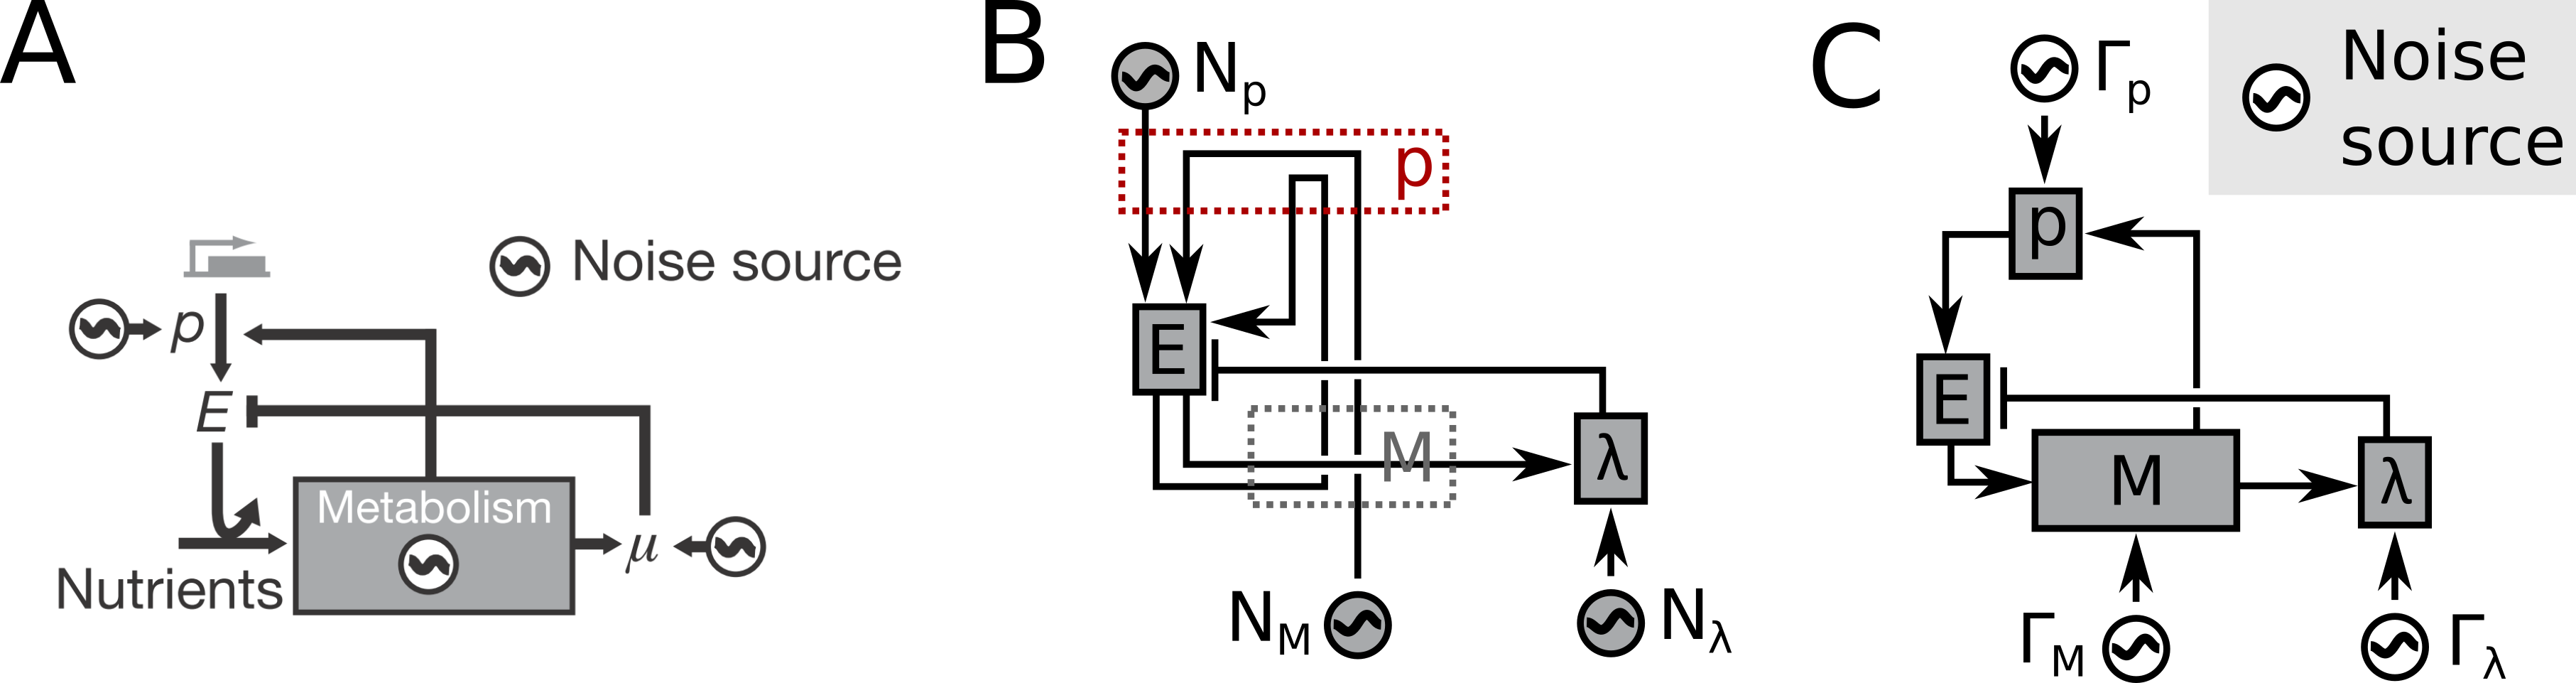
\includegraphics[width=0.9\textwidth]{model_nghe_v2.png}
	\caption{ 
		(A) Original diagram as printed in Kiviet et al. \cite{Kiviet2014}.
		(B) More technical diagram stating the relations between parameters of interest (gray boxes), and noise sources $N_P$, $N_M$, and $N_\lambda$. Arrows indicate how ODEs or functions that describe the parameters of interest are coupled. 
		Arrows that go trough the red dashed box correspond to terms that not only couple the two parameters connected by the arrow, but also make up the parameter $p$ (see also main text).
		Arrows that go through the grey box are arrows which are thought to be biologically connected to the metabolism.
		(C) An alternative version of the model with more parameters modelled explicitly. Noise sources are printed white in this diagram since they are not described by separate ODEs, which was the case in Kiviet et al. \cite{Kiviet2014}. 
	}
	\label{fig:modeldrawing}
\end{figure}

A straight forward way to model a system with these parameters, is writing down an ordinary differential equation (ODE) for each parameter involved. 
%
The Nghe model takes a somewhat different approach (it is more concise), which will be discussed later.
%
The ODEs below relate to the cartoon in Fig. \ref{fig:modeldrawing}.C
and describe the dynamics per parameter:
%
\begin{align}
\label{myfirstequation}
\dot{M} = & - \frac{(M-M_0)}{\tau}  \nonumber \\ 
          & + c_M \cdot \Gamma_M  \nonumber \\ % (1-T_{M\leftarrow E})
          & + T_{M\leftarrow E} \cdot c_M' \cdot (\frac{E}{E_0} - 1)  
\end{align}
% deltaMetabolism = -(metabolismValues(end)-parameters.metabolism0) * 1/parameters.dampingTimeMetabolism + ... % damping; 1 is the equilibrium value
% (1-parameters.transmissionEnzymeMetabolism) * ((rand()-.5)*2) * parameters.noiseSizeMetabolism + ...                              % white noise component
% parameters.transmissionEnzymeMetabolism * (enzymeValues(end)/parameters.enzymeTarget-.5) * parameters.noiseSizeMetabolism;             % noise component due enzyme
%
%
\begin{align}
	\dot{\lambda} = & -\frac{(\lambda - \lambda_0 )}{\tau_\lambda} \nonumber \\ 
 			& + c_\lambda \cdot \Gamma_\lambda \nonumber \\  %  (1-T_{\lambda\leftarrow M}) \cdot
			& + T_{\lambda\leftarrow\ M} \cdot c_\lambda' \cdot (\frac{M}{M_0}-1) 
\end{align}
%
\begin{align}
\label{mythirdequation}
\dot{P} = & - \frac{(P-P_0)}{\tau_P} \nonumber \\ 
		 & + c_p \cdot \Gamma_p \nonumber \\ 
         & + T_{P\leftarrow M} \cdot c_P' \cdot (\frac{M}{M_0}-1)  \nonumber \\ 
         & + R_{P\leftarrow M} \cdot c_P' \cdot (\frac{M}{M_0}-1)
\end{align}
%
\begin{align}
\label{mylastequation}
\dot{E} = P - \lambda E
\end{align}
%
Where $M$ describes the state of the metabolism, $\lambda$ is the growth rate, $P$ is the production rate, $E$ is the amount of enzyme, $\tau$ is a dampening term ($X_0$ is the equilibrium value), $T_{X \leftarrow Y}$ is the noise transmission constant from $X$ towards $Y$, $c_X$ and $c_X'$ are constants that set the size of the fluctuations, $\Gamma_X$ is a white noise source.
$R_{X \leftarrow Y}$ indicates a regulatory interaction, an addition to the model, but this notation is just cosmetic, as $T_\text{effective}=T+R$.
%
This model assumes all parameters have an average value from which fluctuations deviate, but always return. Hence the dampening terms.
With respect to transmission, I furthermore rescale the absolute value of the noise to be comparable to the target noise (hence the $M_0^{-1}$ and $c_X$ terms in combination with the $T_{X\leftarrow Y}$ term).

This is similar to the model that Philipe Nghe suggested in Kiviet et al. \cite{Kiviet2014}, which was inspired by Dunlop et al. \cite{Dunlop2008} (see supplement of that manuscript for a description of the Dunlop model).
%
A difference between my equations, the Nghe equations and the Dunlop equations lies in the dampening terms (those containing $\tau$, $\beta$ or $\mu_E$). In my model noise is effected through the ODE, and dampening occurs on the parameter of interest. In Dunlop et al., there are two dampening terms, one specifically dampening the noise and a second term dampening the parameters of interest. \red{Nghe also takes the latter approach, see below.}
% dampening being effected through the $(-\beta_X \cdot N_X)$ term and the $\mu_E$ parameter (see later for a more involved discussion on these parameters)}.

The correlations between these equations can be found by linearizing them, writing the correlations in Fourier space, and back-transforming them using residue integration techniques. 
\red{These notes do} not fully explores this, but \red{this will partially be discussed later}.
First, a comparison of the above model with the Nghe model is made.

\subsubsection*{Numerical implementation}

Out of practical considerations, we numerically solved Eq. \ref{myfirstequation}-\ref{mylastequation} by simple Euler propagation implemented in Matlab.
%
The script \texttt{growthnoisepropagatorv2.m} will be made available in an online Github repository, parameter settings that were used are shown below.
%
For the dilution mode: 
\begin{gather*}
E_0= 2000,
\mu_0= 1,
%\lambda_0= 0.6931,
\lambda_0= 0.0116, 
\nonumber \\ p_0= 23.1049, 
C_0= 1,
\tau_\lambda= 120,
\Gamma_\lambda= 8.3255e-04,
\Gamma_\lambda'= 8.3255e-04,
\nonumber \\ \tau_p= 120,
\Gamma_p= 0.0048,
\Gamma_p'= 0.0048,
\tau_C= 120,
\Gamma_C= 1.0000e-03,
\Gamma_C'= 1.0000e-03,
%dampingNoiseOnly= Inf,
\nonumber \\ T_{C\rightarrow\lambda}= 0,
T_{C\rightarrow{p}}= 0,
T_{E\rightarrow{C}}= 1,
T_{\lambda\rightarrow{E}}= -1;
%interactionCProduction= 0,
\end{gather*}
%
($\lambda$ is given in units of $min^{-1}$ here.)
For the catabolic mode: 
\begin{gather*}
E_0= 2000,
\mu_0= 1,
%\lambda_0= 0.6931,
\lambda_0= 0.0116,
\nonumber \\ p_0= 23.1049,
C_0= 1,
\tau_\lambda= 60,
\Gamma_\lambda= 0,
\Gamma_\lambda'= 8.3255e-06,
\nonumber \\ \tau_p= 60,
\Gamma_p= 1.5200,
\Gamma_p'= 1.5200,
\tau_C= 60,
\Gamma_C= 0,
\Gamma_C'= 0.3162,
%dampingNoiseOnly= Inf,
\nonumber \\ T_{C\rightarrow\lambda}= 0.9000,
T_{C\rightarrow{p}}= 0,
T_{E\rightarrow{C}}= 0.9000,
T_{\lambda\rightarrow{E}}= -1;
%interactionCProduction= 0,
\end{gather*}
For the common mode: 
\begin{gather*}
E_0= 2000,
\mu_0= 1,
%\lambda_0= 0.6931,
\lambda_0= 0.0116,
\nonumber \\p_0= 23.1049,
C_0= 1,
\tau_\lambda= 6,
\Gamma_\lambda= 0,
\Gamma_\lambda'= 8.3255e-06,
\nonumber \\ \tau_p= 6,
\Gamma_p= 0,
\Gamma_p'= 0.0481,
\tau_C= 60,
\Gamma_C= 0.3162,
\Gamma_C'= 0.3162,
%dampingNoiseOnly= Inf,
\nonumber \\ T_{C\rightarrow\lambda}= 0.9000,
T_{C\rightarrow{p}}= 0.9000,
T_{E\rightarrow{C}}= 0,
T_{\lambda\rightarrow{E}}= -1;
%interactionCProduction= 0,
\end{gather*}
For the combined scenario: 
\begin{gather*}
E_0= 2000,
\mu_0= 1,
%\lambda_0= 0.6931,
\lambda_0= 0.0116,
\nonumber \\p_0= 23.1049,
C_0= 1,
\tau_\lambda= 60,
\Gamma_\lambda= 2.4034e-04,
\Gamma_\lambda'= 2.4034e-04,
\nonumber \\ \tau_p= 60,
\Gamma_p= 0.5308,
\Gamma_p'= 0.5308,
\tau_C= 60,
\Gamma_C= 0.1459,
\Gamma_C'= 0.1459,
%dampingNoiseOnly= Inf,
\nonumber \\ T_{C\rightarrow\lambda}= 0.2700,
T_{C\rightarrow{p}}= 0.3000,
T_{E\rightarrow{C}}= 0.2700,
T_{\lambda\rightarrow{E}}= -1,
%interactionCProduction= -0.2700,
\end{gather*}
%
Cross-correlations were calculated based on 100000 one-minute timesteps, noise was introduced with the matlab function \texttt{normrnd}.
% 
The feedback is added by subtracting $0.27$ from the $T_{C\rightarrow\lambda}$ parameter, i.e. setting it to zero.

\subsection*{Separate noise equations}

Both Nghe and Dunlop define separate ODEs for the noise terms:
%
\begin{align}
\label{eq:generalgillespienoise}
\dot{N}_X = \sqrt{C_X} \cdot \Gamma_X - N_X/\tau
,
\end{align}
%
though their notation might be slightly different (I used Daniel Gillespie's notation \cite{Gillespie1996}; a capital C is used here to follow Gillespie's square root notation, $\sqrt{C_X}=c_x$).
With for our case $X$ equaling $\lambda$, $M$ or $P$. Note that $\tau^{-1}=\beta$ ($\beta$ is used in Nghe and Dunlop).

Not so relevant for our case, but noteworthy, is that in the Dunlop model, which models a completely different process than the one described here \cite{Dunlop2008}, the \textit{solutions} of the ODEs describing the noise are plugged into the ODEs describing the protein dynamics. This leads to an additional memory effect.
%
That is:
%
\begin{align}
\label{dunlopgeneralequation}
\dot{X} = & N_X  + F(X) + X/\tau
,
\end{align}
%
with $F(X)$ some arbitrary function of $X$. 
Note that the $N_X$ function also contains a $\tau$ term (see Eq. \ref{eq:generalgillespienoise}), which is effectively integrated, thus leading to effects of the fluctuations much longer timescales than $\tau$. 
This effect is (partially) countered by the third term in Eq. \ref{dunlopgeneralequation}, which also contains the $\tau$ term.

\subsection*{Nghe model}

As mentioned, the Nghe model takes a different approach. 
The formulae that follow correspond to Fig. \ref{fig:modeldrawing}.B (Fig. \ref{fig:modeldrawing}.A contains the version of the cartoon which was published in Kiviet et al.).
The starting point,
%
\begin{align}
\label{eq:Nghe1}
\dot{E} = P - \lambda E
,
\end{align}
%
is the same in my model, but after linearization (defined as $X=X_0+\delta X$) this leads to only one ODE:
% CONVENIENT NOTE TO SELF: %%%%%%%%%%%%%%%%%%%%%%%%%%%%%%%%%%%%%%%%%%%
% See written notes from 28.9.2016 for explicit linearization.
% END CONVENIENT NOTE TO SELF: %%%%%%%%%%%%%%%%%%%%%%%%%%%%%%%%%%%%%%%
%
\begin{align}
\label{eq:ODEElinearized}
\frac{ \delta{\dot{E}} }{E_0 \mu_0} 
+ \frac{\delta E}{E_0} 
%& = 
%\left[
% T_{E \leftarrow E} \frac{\delta E}{E_0} + T_{E \leftarrow G} N_G + N_E 
% \right]
% + T_{E \leftarrow \mu} \frac{\delta \mu}{\mu_0} \nonumber \\
& =
\frac{\delta p}{E_0 \mu_0} + T_{E \leftarrow \mu} \frac{\delta \mu}{\mu_0}
.
\end{align}
%
Noise terms are introduced with ODEs that are also shown above in Eq. \ref{eq:generalgillespienoise}.
 Additionally, two functions are defined for $p$ and $\lambda$. These are not ODEs, as the effects on these parameters are thought to happen on fast timescales. The parameters are however linearized (and thus written as $\delta X$). The equation
%
\begin{align}
\label{eq:Nghe3}
\frac{\delta\mu}{\mu_0} = T_{\mu \leftarrow E} \frac{\delta E}{E_0} + T_{\mu \leftarrow G} N_G + N_\mu
\end{align}
%
simply defines the evolution of $\delta \mu$.
There is also a similar equation for $\delta p$:
%
\begin{align}
\label{eq:Nghe4}
\frac{\delta{p}}{E_0 \mu_0} = T_{E \leftarrow E} \frac{\delta E}{E_0} + T_{E \leftarrow G} N_G + N_E
,
\end{align}
%
which plays a bit more complicated role.
It is defined using terms that pertain to E, like $T_{E \leftarrow G}$, such that it can be directly plugged into Eq. \ref{eq:ODEElinearized}. 
Indeed, plugging Eq. \ref{eq:Nghe4} into Eq. \ref{eq:ODEElinearized} leads to equation:
%
\begin{align}
\label{eq:Nghe5}
\frac{ \delta{\dot{E}} }{E_0 \mu_0} 
+ \frac{\delta E}{E_0} 
& = 
\left[
 T_{E \leftarrow E} \frac{\delta E}{E_0} + T_{E \leftarrow G} N_G + N_E 
 \right]
 + T_{E \leftarrow \mu} \frac{\delta \mu}{\mu_0} 
\end{align}
%
which corresponds to equation 5 in the Kiviet et al. \cite{Kiviet2014} manuscript.
I say it is a bit complicated, since Eq. \ref{eq:Nghe4} has no role in the model (we could also just have defined Eq. \ref{eq:Nghe5} immediately), except that it shows us which part of the model can be interpreted as being the production rate.
This is also the reason why $p$ is depicted as a red dashed box in Fig. \ref{fig:modeldrawing}.

%
%{\color{red}
%There are currently a few things unclear about Eq. \ref{eq:Nghe3} and Eq. \ref{eq:Nghe4} (respectively Eq. 3 and 4 in the Kiviet et al. manuscript):
%\begin{itemize}
%\item It seems that the transmission terms $T_{X\leftarrow Y}$ state how the parameter of interest ($X$) is affected by another parameter of interest ($Y$), however, for this to be true, the left-hand side parameter should match the first parameter in the subscript of $T$. E.g. how can a $T_{E\leftarrow G}$ term appear in the equation for $\delta p$ and moreover, what does the term $T_{E \leftarrow E}$ mean?
%\item It is not clear to me how these formulae relate to the diagram that was drawn (see Fig. \ref{fig:modeldrawing}). Why is E directly effecting $\mu$? Should there not also be a metabolism term $G$ or $\delta G$? Also why does the formula for $\delta p$ contain transmission from $E$ (assuming $T_{E\leftarrow E}$ was a type and should have been $T_{p\leftarrow E}$)? Why does the formula for $\delta p$ contain a noise term for E (ie. $N_E$)?
%\item These are not ODEs (which would seem more natural to me), probably this is intended this way, and the relationship between the parameters is defined as such. (And could be derived from ODEs.)    
%\end{itemize}
%%I am currently not sure how these equations relate to my own equations, as subscripts in Eq. \ref{eq:Nghe4} seem inconsistent with the fact that transmission should be towards $P$ (e.g. what is $T_{E\leftarrow E}$?).
%}
%
%In any case, given that noise and other parameters are related in terms of parameters (not derivatives), the following formulae are probably underlying the Nghe model:
%
%\begin{align}
%\dot{M} = & \dot{N}_M  \nonumber \\ 
%& + T_{M\leftarrow E} \cdot c_M \cdot (\frac{E}{E_0} - 1)  
%\end{align}
%
%\begin{align}
%\dot{\lambda} = & \dot{N}_\lambda \nonumber \\ 
%& +    T_{\lambda \leftarrow M} \cdot c_\lambda \cdot (\frac{M}{M_0}-1) 
%\end{align}
%
%\begin{align}
%\dot{P} = & \dot{N}_P \nonumber \\ 
%& + T_{P\leftarrow M} \cdot c_P \cdot (\frac{M}{M_0}-1)  \nonumber \\ 
%& + R_{P\leftarrow M} \cdot c_P \cdot (\frac{M}{M_0}-1)
%\end{align}
%
%Where the normalizations by $X_0$ were left out again.

Note that dampening terms can be implicitly present in the Nghe model, in the form of a transmission from the parameter to itself.
Specifically, $T_{E \leftarrow E}$ can fulfill this role. % when it is negative and $<1$. 
Second order dampening can also occur, 
as is pointed out in the Kiviet et al supplementary information, which states that the time scale of the $E$ fluctuations is set by the term $\mu_0(1-T_{E \leftarrow \mu}T_{\mu \leftarrow E}-T_{E \leftarrow E})$.

% I previously thought that dampening was not present in the Nghe model, but this is not the case.
% Here the previous text:
%Note however, that this results in the absence of dampening terms on the parameters $X$ themselves, which might lead to 
%%non-steady state behavior of the parameters.
%unstable behavior of the parameters.
%The term $X/\tau$ could be added to each of the equations to resolve this issue; the term $-N_X/\tau$ from the noise ODEs could then be dropped.
%{\color{red}Note that a $\mu_E$ term appears eventually in Nghe's equations, which might play the role of a second dampening term.}



%%%%%%%%%%%%%%


 % This used to be a separate chapter, but is now included as notes to the CRP chapter


\subsection*{III. The Towbin et al. model equations}

\subsubsection*{The equations}


This supplementary note offers a brief overview of the formulae used in Towbin et al. to describe the CRP regulation system, and its relation to metabolite concentrations and growth.
%
This is meant as a reference, to allow comparison between the linearized noise model that was used in this chapter to model the dynamics of metabolism and growth (described in supplementary note II), and a more sophisticated model of the biochemical network that is aimed to model the population average response to changes in the extracellular environment. 
%
These equations are directly taken from the supplementary notes of Towbin et al. (Equations 7-9), except that some parameter symbols have been changed to match our notation \cite{Towbin2017}.
%
The equations are the following:
%Towbin et al. suggest the following set of equations:

\begin{align}
	\label{eq:TB:dotM}
	\dot{C_M} & = \lambda ( \frac{k_f}{k_f+x} - C_M) ,\\
%\end{align}
%\begin{align}
	\label{eq:TB:dotx}
	\dot{x} & = \frac{\alpha}{k_2} \left(    \beta f_M(C_M) \frac{k_1}{x+k_1}  -    \lambda    \right) ,\\
%\end{align}
% renamed p_BT to alpha
%\begin{align}
	\label{eq:TB:mu}
	\lambda & =\gamma(1-C_M) \frac{x}{x+k_2}
	.
\end{align}

Here, $C_M$ represents the metabolic enzyme expression, $x$ the pool of carbon metabolites which give feedback to the CRP system, and $\lambda$ the cellular growth rate\footnote{
    In this chapter, we use both the symbols $\lambda$ and $\mu$ to indicate growth rate,
    $\lambda$ when the units are $/\text{min}$ and
    $\mu$ when the units are $\text{doublings}/\text{hour}$.}.
%
Furthermore, $k_1$, $k_2$, and $k_f$ are Michaelis Menten rate constants, where $k_1$ pertains to carbon import (which is self-inhibited), $k_2$ to biomass production and $k_3$ to feedback by metabolites.
%
$\alpha$, $\beta$ and $\gamma$ are also constants, 
$\alpha$ sets the conversion ratio between metabolite consumption and growth,
$\beta$ the maximum import rate of metabolites,
and $\gamma$ the maximum catalytic rate of ribosomes.
%$\gamma$ maximum catalytic rate of ribosomes.
%$\alpha$ is a constants, which set the conversion ratio between metabolite consumption and growth, and $\beta$ is a constant that sets the maximum import rate of metabolites.
% which determine the conversion rate from metabolites to biomass.
%
$f_M(C_M)$ is a function of $C_M$, which describes \lq{the regulation of the limiting enzyme for carbon uptake and catabolism by CRP}\rq{} \cite{Towbin2017}. 
%
The left and right terms (within brackets) in Eq. \ref{eq:TB:dotM} relate to production and dilution and in Eq. \ref{eq:TB:dotx} the left and right terms in brackets relate to import and consumption.
%
The growth rate is a function of metabolite consumption and ribosome concentration $C_R=1-C_M$.

\subsubsection*{Graphic representations of the model}

The relationships that are set in the differential equations are presented in a diagram in figure \ref{fig:CRP:benjamin_ODEs_diagram}.
%
The contributions of the left and right terms can be plotted separately to understand the dynamic behavior of the system when these terms change independently, see figure \ref{fig:CRP:benjamin_ODEs}.

%%%%%%%%%%%%%%%%%%%%%%%%%%%%%%%%%%
\begin{figure}
	\centering
	\includegraphics[width=0.5\textwidth]{CRP-figXsup_BenjaminInteractions_v2.pdf}
	\caption{ 
		\textbf{Diagram of Towbin et al. ODE model.}
		This diagram shows how the parameters in the Towbin et al. model relate to each other. $C_M$ and $x$ are the metabolic enzyme and metabolite concentration respectively, which are both modeled using differential equations. The ribosome concentration is only implicitly present as $C_R=1-C_M$. Metabolic enzyme production $p_m$, growth rate $\lambda$, metabolite production/import rate $p_x$ and metabolite consumption are all terms that are part of these differential equations.
	}
	\label{fig:CRP:benjamin_ODEs_diagram}
\end{figure}
%%%%%%%%%%%%%%%%%%%%%%%%%%%%%%%%%%


%%%%%%%%%%%%%%%%%%%%%%%%%%%%%%%%%%
\begin{figure}
	\centering
	\includegraphics[width=0.8\textwidth]{pdf_benjamin_ODE_relations.pdf}
	\caption{ 
		\textbf{Using models to understand the dynamic behavior of stochastic metabolic and growth fluctuations.}
		(Left) Illustrations of the contributions from the positive (production) and negative (dilution) terms to the differential equation that describes the time evolution of the concentration of metabolic enzymes as a function of that concentration $C$, according to the Towbin et al. model \cite{Towbin2017}. The different lines correspond to different values of the metabolite concentration $x$ ($x={0.9, 1.0, 1.1}$). 
		(Right)	Similar as on the left, except that the terms are production and consumption of metabolites as a function of metabolite concentration $x$ and that the different lines correspond to different values of the metabolic enzyme concentration $C$ ($C={0.45,0.50,0.55}$). (Towbin et al. focus on import of metabolites as rate limiting step in the rate at which they are created, but we have used the more general term production here.) 
		These plots are merely to illustrate the systems behavior, so all parameter values were simply set to $1$.
		%, the parameter values used for plotting are: 
		%$k_1=1$,
		%$k_2=1$,
		%$k_f=1$,
		%$\beta=1$,
		%$\gamma=1$ and
		%$\alpha=1$.
		%
		%  mu0 = .25;
		%  C0=.5; C = [C0*.9, C0, C0*1.1] = 0.4500    0.5000    0.5500
		%  x0=1; x = [x0*.9,x0,x0*1.1]
		%
		%
	}
	\label{fig:CRP:benjamin_ODEs}
\end{figure}
%%%%%%%%%%%%%%%%%%%%%%%%%%%%%%%%%%






\clearpage
\FloatBarrier
\section*{Supplementary figures}
\setheader{Supplementary figures}

%%%%%%%%%%%%%%%%%%%%%%%%%%%%%%%%%%%%%%%%%%%%%%%%%%%%%%%%%%%%%%%%%%%%%%%%%%%%%%%%%%%%%%%%%%%%%%%%%%%%%%%%%%%%%%%%%%%%%%%%%%%%%%%%%%%%%%%%%%%%%%%%%%%%%%%%%%%%%%%%%%%%%%%%%%%%%%%%%%%%%%%%%%%%%%%%%%%%%%%%%%%%%%%%%
%Sup belonging to figure 1 %%%%%%%%%%%%%%%%%%%%%%%%%%%%%%%%%%%%%%%%%%%%%%%%%%%%%%%%%%%%%%%%%%%%%%%%%%%%%%%%%%%%%%%%%%%%%%%%%%%%%%%%%%%%%%%%%%%%%%%%%%%%%%%%%%%%%%%%%%%%%%%%%%%%%%%%%%%%%%%%%%%%%%%%%%%%%%%%%%%%%%%%%%%%%%%%%%%%%%%%%%%%%%%%%

\begingroup % note that this is needed such that captionof not mess up indentation
\begin{figure}%%%%%%%%%%%%%%%%%%%%%%%%%%%%%%%%%%
	\centering
	\includegraphics[width=1.0\textwidth]{CRP-figXsup_overviewRegulationTCA.pdf}
	\clearpage % insert a page break	
\end{figure}	

\clearpage

\captionof{figure}{    
	\textbf{Regulation of the TCA cycle and ED pathway.} 
	Some regulatory proteins control the expression of many tricarboxylic acid (TCA) cycle and/or enzymes glycolysis pathway simultaneously.
	This diagram shows the regulatory effects of CRP, but also of the Catabolite repressor activator (Cra) and the Anoxic redox control A (ArcA) protein.
	Cra controls the direction of the metabolite flux through metabolic pathways \cite{Keseler2017, Ramseier1995}. Cra is activated by the metabolite fructose-1,6-bisphosphate \cite{Kochanowski2013a}.
	ArcA is part of a two component system (ArcAB) which controls gene expression in response to aerobic versus anaerobic conditions \cite{Keseler2017, Alvarez2010}.
	Metabolites are displayed in larger font, enzymes that catalyze reactions in smaller fonts.
	In the colored boxes, regulation by CRP is displayed by an oval symbol marked "CRP".
	Similarly, when an enzyme is regulated by Cra or ArcA this is displayed next to the boxes; a plus or minus symbol indicates positive or negative regulation.
	Additionaly, in the boxes this diagram displays the concentration of particular enzymes in ppm, as annotated in PaxDb (retrieved in 2015) \cite{Wang2015}.
	The boxes are also color-coded according to abundance of the enzymes.
	The diagram is based on EcoCyc \cite{Keseler2017}. 
	From top to bottom, clockwise, enzymes abbreviations stand for glucose 6-phosphate, fructose 6-phosphate, fructose 1,6-biphosphate, glyceraldehyde 3-phosphate, 1,3-biphospho-D-glycerate, 3-phospho-glycerate, 2-phospho-glycerate, phosphoenolpyruvate, pyruvate, acetyl coenzyme A, citrate, cis-aconitate, d-threo-isocitrate, (succinate, glyoxalate, acetyl-CoA), 2-oxo-glutarate, succinyl-CoA, succinate, fumarate, malate, oxaloacetate.
    \label{fig:CRP:figOverviewTCARegulation}
	% See also: https://biocyc.org/ECOLI/NEW-IMAGE?type=PATHWAY&object=TCA
	% And: https://biocyc.org/ECOLI/NEW-IMAGE?type=PATHWAY&object=GLYCOLYSIS
}%%%%%%%%%%%%%%%%%%%%%%%%%%%%%%%%%%%%%%%%%%%%%%%
\endgroup

%%%%%%%%%%%%%%%%%%%%%%%%%%%%%%%%%%%%%%%%%%%%%%%%%%%%%%%%%%%%%%%%%%%%%%%%%%%%%%%%%%%%%%%%%%%%%%%%%%%%%%%%%%%%%%%%%%%%%%%%%%%%%%%%%%%%%%%%%%%%%%%%%%%%%%%%%%%%%%%%%%%%%%
%%%%%%%%%%%%%%%%%%%%%%%%%%%%%%%%%% cAMP optimality curve me & Benjamin
\begingroup % note that this is needed such that captionof not mess up indentation
\begin{figure}
    \centering
    \includegraphics[width=0.49\textwidth]{pdf_optimalityCurve.pdf}
    \caption{ 
        \textbf{Optimum curve based on bulk measurements.}
%        \textbf{Growth rates in minimal medium supplemented with lactose at different cAMP concentrations.}
        The black line with solid black squares indicates
        exponential phase growth rates of $\Delta$cAMP cells at different concentrations of cAMP as measured in a platereader that measured bacterial density over time.
        %
        The growth rate was determined by an exponential fit, based on a manually selected part of the bacterial density curve that displayed exponential growth.
        %
        We also used an alternative method to determine growth rates (gray dashed line), were we 
        fitted an exponential to part of the bacterial density curve that fell between two threshold values.
        We consider this less reliable, as growth is not guaranteed to be exponential.
        %
        We also show the optimum curve as measured by Towbin et al \cite{Towbin2017} (dashed blue line),
        who calculated growth rate based on an exponential fit to a two hour window,
        which was selected by an algorithm that looked for the longest period of stable growth rate.        
        %
%        Method 1 refers to a procedure where the fit range was manually chosen, whereas in method 2 the fits were made inbetween certain OD values.
%        Also, this figure shows data from a similar experiment performed by Towbin et al. \cite{Towbin2017}.
        %        1 is manual selection of data that fit is bas
    }
    \label{fig:CRP:ocurvePlatereader}
\end{figure}
%%%%%%%%%%%%%%%%%%%%%%%%%%%%%%%%%%
\endgroup

%%%%%%%%%%%%%%%%%%%%%%%%%%%%%%%%%%%%%%%%%%%%%%%%%%%%%%%%%%%%%%%%%%%%%%%%%%%%%%%%%%%%%%%%%%%%%%%%%%%%%%%%%%%%%%%%%%%%%%%%%%%%%%%%%%%%%%%%%%%%%%%%%%%%%%%%%%%%%%%%%%%%%%
%%%%%%%%%%%%%%%%%%%%%%%%%%%%%%%%%% cartoons of constructs


\begin{figure}
    \centering
    \includegraphics[width=1.0\textwidth]{CRP-fig0sup.pdf}
    \caption{ 
        \textbf{The reporters used in this study.}
        (Top left panel) This panel shows the lac operon, on which these promoters are based.
        The lac operon consists of three genes, \textit{lacZ}, \textit{lacY} and \textit{lacA}, that are required to metabolize lactose.
        These three genes are regulated by the same promoter, which is activated by CRP. 
        When there is no lactose, transcriptional repressor lacI blocks gene expression from the lac operon.
        The \textit{lacI} gene is encoded at a location near to the lac operon, and is also displayed (it is also regulated by CRP).
        When there is lactose, transcriptional repressor lacI is inhibited by lactose and LacZ, LacY and LacA are produced.
        CRP recruits initiation factor sigma 70, which is followed by polymerase binding and transcription.
        (It is furthermore also known that pleiotropic transcription factor H-NS can bind to the lac operon and repress gene expression.)
        (Top right and bottom left panel) Using the lac promoter as a starting point, Towbin et al. created two reporters \cite{Towbin2017}.
        Both posses mutations which result in the removal of the LacI binding site (indicated with a black cross).
        The CRP sensitive promoter is then created by fusing the promoter to a GFP fluorescent protein sequence.
        We call this the CRP reporter or metabolic reporter.
        In the promoter of the second reporter, which is intented to measure background fluctuations in gene expression, also mutations have been introduced that remove the CRP binding site. Instead, a consensus binding site for the sigma 70 initiation factor is introduced, effectively making it a constitutive promoter that is otherwise similar to the promoter used for the CRP reporter. It was also fused to GFP, and we call this the sigma 70 reporter or constitutive reporter.
        (Bottom right panel) To be able to perform single cell measurements that involve both reporters, we replaced the GFP sequences of the metabolic and constitutive reporters with mVenus and mCerulean sequences respectively. 
        The GFP reporters were introduced to cells using plasmids as vector,
        whilst the mVenus and mCerulean reporters were chromosomally inserted at the \textit{intC} and \textit{galK} locations respectively.
    }
    \label{fig:CRP:fig0sup}
\end{figure}



%%%%%%%%%%%%%%%%%%%%%%%%%%%%%%%%%%%%%%%%%%%%%%%%%%%%%%%%%%%%%%%%%%%%%%%%%%%%%%%%%%%%%%%%%%%%%%%%%%%%%%%%%%%%%%%%%%%%%%%%%%%%%%%%%%%%%%%%%%%%%%%%%%%%%%%%%%%%%%%%%%%%%%%%%%%%%%%%%%%%%%%%%%%%%%%%%%%%%%%%%%%%%%%%%
%% Pulsing dynamics

\begin{figure}%%%%%%%%%%%%%%%%%%%%%%%%%%%%%%%%%%
	\centering
	\includegraphics[width=9cm]{png_averagetimetraces_4.png} 
	\includegraphics[width=9cm]{png_averagetimetraces_2.png}
	\includegraphics[width=9cm]{png_averagetimetraces_5.png}
	%\clearpage % insert a page break
%\end{figure}	
%
%\clearpage
%
%\captionof{figure}{ 
\caption{   
	\textbf{Additional time traces from the cAMP pulsing experiment.} 
	This figure displays additional data for figure \ref{fig:CRP:fig1}. 
	It shows time traces for parameters measured in a population of $\Delta$cAMP cells (blue dots are single cell measurements, the black line is the population average) that were grown alternately in minimal medium supplemented with 43 $\upmu$M cAMP and minimal medium supplemented with 2100 $\upmu$M cAMP.
	Red and green dotted lines indicate times where the concentration was switched, as indicated in the legend.
	For this experiment, also the production rate of the metabolic reporter was determined (top panel).	
	Furthermore, also the production rate and concentration of a constitutive reporter where determined (bottom two panels), see main text for more on these quantities.	
   	\label{fig:CRP:fig1sup}
}
%}
\end{figure}%%%%%%%%%%%%%%%%%%%%%%%%%%%%%%%%%%%%%%%%%%%%%%%


\begin{figure}%%%%%%%%%%%%%%%%%%%%%%%%%%%%%%%%%%%%%%%%%%%%%%% Figure plotting cAMP input signal vs. growth
    \centering
    \includegraphics[width=12cm]{pdf_cAMPvsGrowth.pdf}
    \caption{ 
        \textbf{Growth rates during the pulsing experiment against cAMP concentration}. 
        This plot shows the population average growth rate of $\Delta$cAMP cells during the pulsing experiment (see main text).
        In the left panel the growth rates are shown from the regime where the cAMP concentration in the medium was switched every hour between low and high concentrations (43 and 2100 $\upmu$M respectively), 
        and in the right panel data is shown from the regime where the cAMP concentration switched every five hours.
        Note that these cells are not in steady state. 
        Growth rates are not only determined by the cAMP concentration, 
        but also by the history of the population.
    }
    \label{fig:CRP:pulsingCAMPVsMu}
\end{figure}%%%%%%%%%%%%%%%%%%%%%%%%%%%%%%%%%%%%%%%%%%%%%%%


\begin{figure}%%%%%%%%%%%%%%%%%%%%%%%%%%%%%%%%%%%%%%%%%%%%%%%
	\centering
	\includegraphics[width=0.75\textwidth]{pdf_timeevolution_2.pdf}	
	\includegraphics[width=0.75\textwidth]{pdf_timeevolution_3.pdf}
	\includegraphics[width=0.75\textwidth]{pdf_timeevolution_4.pdf}	
	%\clearpage % insert a page break	
%\clearpage
\caption{%of{figure}{    
		\textbf{Time evolution of production versus growth rate during block pulses of high and low cAMP concentrations.}
		(Top) The production rate of the CRP reporter plotted against growth rate, color coded for time. Production is determined here by the difference in absolute signal between two timepoints, divided by the amount of time inbetween these two points and divided by the area of the cell. Note that the production rate might also depends on the growth rate, as does the final concentration of the protein. This makes this data not trivial to interpret.
		(Middle) Similar to top panel, but production rate is divided by growth rate, since production rates might be more faithfully represented as fractions of the growth rate.
		(Bottom) Similar to top panel, but production rate is divided by the production rate of the constitutively expressed label, which serves a reference for the total production rate capacity of the cell.
        \label{fig:CRP:productiontimeevolutions}
}
\end{figure}%%%%%%%%%%%%%%%%%%%%%%%%%%%%%%%%%%%%%%%%%%%%%%%

\begin{figure}%%%%%%%%%%%%%%%%%%%%%%%%%%%%%%%%%%%%%%%%%%%%%%% SCATTERS f(CRP,MU) and f(const, mu)
	\centering
	\includegraphics[width=0.75\textwidth]{pdf_timeevolution_5.pdf}
	\caption{ 
		\textbf{Time evolution of metabolic reporter concentration normalized by constitutive reporter concentration.}
		This figure is similar to figure \ref{fig:CRP:productiontimeevolutions}, but shows the concentration of the metabolic reporter divided by the constitutive reporter on the x-axis, instead of production rates.
	}
	\label{fig:CRP:normalizedconcentrationtimeevolutions}
\end{figure}%%%%%%%%%%%%%%%%%%%%%%%%%%%%%%%%%%%%%%%%%%%%%%%


% pdf_scattersoftraces_1

\begin{figure}%%%%%%%%%%%%%%%%%%%%%%%%%%%%%%%%%%%%%%%%%%%%%%% SCATTERS f(CRP,MU) and f(const, mu)
	\centering
	\includegraphics[width=0.37\textwidth]{png_scattersoftraces_1.png}
	\includegraphics[width=0.37\textwidth]{png_scattersoftraces_2.png}	
	\caption{ 
		\textbf{Scatter plots of growth rate versus metabolic and constitutive reporter from single cell measurements.}
        These plots relate to the pulsing experiment with \dcamp cells, figure \ref{fig:CRP:fig1} in the main text.
		Every point in these plots corresponds to a single cell observation on growth rate and fluorescent label concentration
        that was made during a time series of pulses of high and low concentrations of cAMP.
%        Note that these points come from a time series where the concentration of extracellular cAMP was not constant.
		On the left, growth rate plotted against the concentration of the metabolic reporter.
		On the right, growth rate plotted against the concentration of a constitutive reporter based on the same lac metabolic reporter but with the CRP binding site replaced by a $\upsigma$70 consensus binding site.
		The black lines indicate the average signal for corresponding concentrations and standard deviations.
		The red lines are interpolated 2nd degree polynomial fits of the displayed mean values.
		The red square shows the maximum value of the interpolated values at a metabolic reporter concentration of 225 a.u. (corresponding to a growth rate of 0.63 doublings/hr).
	}
	\label{fig:CRP:scatterspulsing}
\end{figure}%%%%%%%%%%%%%%%%%%%%%%%%%%%%%%%%%%%%%%%%%%%%%%%


\begin{figure}%%%%%%%%%%%%%%%%%%%%%%%%%%%%%%%%%%
	\centering
	\includegraphics[width=0.75\textwidth]{pdf_timetracesinglecell13.pdf}
	\includegraphics[width=0.75\textwidth]{pdf_timetracesinglecell49.pdf}
	\includegraphics[width=0.75\textwidth]{pdf_timetracesinglecell144.pdf}
%	\clearpage % insert a page break	
%\clearpage
%\captionof{figure}{
    \caption{    
	\textbf{Time evolution of growth rate and metabolic reporter concentration for single cells.}
	Each panel is identical to main figure \ref{fig:CRP:fig1}.C, except that each panel corresponds to the behavior of a lineage of single cells.
}
\label{fig:CRP:timevolutionCRPgrowthsinglecell}
\end{figure}%%%%%%%%%%%%%%%%%%%%%%%%%%%%%%%%%%%%%%%%%%%%%%%


%%%%%%%%%%%%%%%%%%%%%%%%%%%%%% Overview (grey bars) with summary parameters from different conditions
% Figure with floating caption

\begingroup % note that this is needed such that captionof not mess up indentation
\begin{figure}
	\centering
	\includegraphics[width=1.0\textwidth]{pdf_chromo1prime_overview_means.pdf}
	\clearpage % insert a page break	
\end{figure}	

\clearpage

\captionof{figure}{    
	\textbf{Comparison of population averages of different parameters in different experimental conditions.} 
	This figure shows growth rates (doublings per hour), production rates (a.u./(px min)), concentrations (a.u./px) and coefficients of variations (CV). 
	C is the abbreviation used for the constitutive reporter (which uses a cyan mCerulean label), and Y is the abbreviation used for the metabolic reporter (which uses a yellow mVenus label).
	WT stands for wild type, indicating wild type cells except the addition of our metabolic and constitutive reporter constructs.
	No FB stands for no feedback, indicating the $\Delta$cAMP cells that also carry the metabolic and constitutive reporter constructs.
	Low, med and high correspond to extracellularly provided cAMP concentrations of 80, 800 and 5000 $\upmu$M cAMP respectively.
	Bars are averages over multiple experiments, and each open circle corresponds to a value observed in one experiment.
    \label{fig:CRP:overviewsummaryparams}
}
\endgroup

%%%%%%%%%%%%%%%%%%%%%%%%%%%%%%



%%%%%%%%%%%%%%%%%%%%%%%%%%%%%%%%%%%%%%%%%%%%%%%%%%%%%%%%%%%%%%%%%%%%%%%%%%%%%%%%%%%%%%%%%%%%%%%%%%%%%%%%%%%%%%%%%%%%%%%%%%%%%%%%%%%%%%%%%%%%%%%%%%%%%%%%%%%%%%%%%%%%%%%%%%%%%%%%%%%%%%%%%%%%%%%%%%%%%%%%%%%%%%%%%
%Sup belonging to figure 2 %%%%%%%%%%%%%%%%%%%%%%%%%%%%%%%%%%%%%%%%%%%%%%%%%%%%%%%%%%%%%%%%%%%%%%%%%%%%%%%%%%%%%%%%%%%%%%%%%%%%%%%%%%%%%%%%%%%%%%%%%%%%%%%%%%%%%%%%%%%%%%%%%%%%%%%%%%%%%%%%%%%%%%%%%%%%%%%%%%%%%%%%%%%%%%%%%%%%%%%%%%%%%%%%%



%%%%%%%%%%%%%%%%%%%%%%%%%%%%%%%%%% Scatters of production
\begin{figure}
	\centering
	\includegraphics[width=1.0\textwidth]{CRP-fig2sup_v2.pdf}
	\caption{ 
	\textbf{Scatter plots of production rates against growth rate.}
	(A) Colored dots show single cell growth rate values plotted against respective single cell production rates of metabolic reporter, which is a proxy for the production rate of metabolic enzymes. 	
	Dots correspond to data points from WT cells with endogenous negative metabolic feedback, and $\Delta$cAMP cells which have been grown at concentrations of 80, 800 and 5000 $\upmu$M cAMP 
	(colored blue, and red, green and orange, respectively).
    The white lines show predicted population average behavior based on a model described in supplementary note I.
	The black lines show the average growth rate for cells that are binned according to production rates, and the black isolines reflect kernel density estimates of the probability distribution (using the matlab function \texttt{kde2d} \cite{Botev2010}).
	The circles with thick black edges show population average values per experiment.
	(B) As panel A, except that this panel shows the relationship between growth and the production rate of a constitutive reporter. 	
	}
	\label{fig:CRP:fig2sup}
\end{figure}
%%%%%%%%%%%%%%%%%%%%%%%%%%%%%%%%%%

%%%%%%%%%%%%%%%%%%%%%%%%%%%%%%%%%% Scatters of conc-conc and prod-prod
\begin{figure}
	\centering
	\includegraphics[width=1.0\textwidth]{png_chromo1prime_overview_custom_scatter_concentrationVsConcentrationYC_withAvgLine.png}
	\includegraphics[width=1.0\textwidth]{png_chromo1prime_overview_custom_scatter_rateVsRateYC_withAvgLine.png}	
	\caption{ 
		\textbf{Concentration-concentration and production-production relationships between metabolic and constitutive reporters.}
    	This figure is similar to Figure \ref{fig:CRP:fig2sup}, except that the relationships plotted are different.
      	Blue, red, green and orange dots again correspond respectively to data points from WT cells with endogenous negative metabolic feedback, and $\Delta$cAMP cells which have been grown at concentrations of 80, 800 and 5000 $\upmu$M cAMP.
		(Top panel) Scatter plots for concentration of metabolic (CRP) reporter against the concentration of constitutive reporter.
        The white line reflects the fact that the sum of the concentrations of the two reporters remains constant 
        (not that the axes are log-log scale; this line would be straight on a linear scale).
		(Bottom panel) Scatter plots for production rate of metabolic reporter against the production rate of constitutive reporter.
        The white line is based on the optimum curve and a simple model describing the relationship between production rate, concentration and growth, 
        see supplementary note I.
	}
	\label{fig:CRP:fig3scatters_CC_pp}
\end{figure}
%%%%%%%%%%%%%%%%%%%%%%%%%%%%%%%%%% 



%%%%%%%%%%%%%%%%%%%%%%%%%%%%%%%%%%%%%%%%%%%%%%%%%%%%%%%%%%%%%%%%%%%%%%%%%%%%%%%%%%%%%%%%%%%%%%%%%%%%%%%%%%%%%%%%%%%%%%%%%%%%%%%%%%%%%%%%%%%%%%%%%%%%%%%%%%%%%%%%%%%%%%%%%%%%%%%%%%%%%%%%%%%%%%%%%%%%%%%%%%%%%%%%%
%Sup belonging to figure 3 %%%%%%%%%%%%%%%%%%%%%%%%%%%%%%%%%%%%%%%%%%%%%%%%%%%%%%%%%%%%%%%%%%%%%%%%%%%%%%%%%%%%%%%%%%%%%%%%%%%%%%%%%%%%%%%%%%%%%%%%%%%%%%%%%%%%%%%%%%%%%%%%%%%%%%%%%%%%%%%%%%%%%%%%%%%%%%%%%%%%%%%%%%%%%%%%%%%%%%%%%%%%%%%%%

%%%%%%%%%%%%%%%%%%%%%%%%%%%%%%%%%%
\begin{figure}
	\centering
	\includegraphics[width=0.8\textwidth]{CRP-fig3sup.pdf}
	\caption{ 
		\textbf{Cross-correlations for non-optimal cAMP expression levels.}
		Also for the non-optimal concentrations of cAMP, 80 $\upmu$M ("low") and 5000 $\upmu$M ("high") respectively, the cross-correlations were determined both for the metabolic and constitutive reporters.
		Colored lines indicate concentration-growth correlations, whereas black lines indicate production-growth correlations.
		The shaded lines are experiments from independent colonies, whereas the dark lines indicate the average over those experiments.
		(A) At lower than optimal cAMP concentrations, we see a similar pattern for the metabolic reporter as at cAMP concentrations of 800 $\upmu$M (figure \ref{fig:CRP:fig3}.B), namely positive correlations between growth and expression of metabolic proteins.
		(B) At higher than optimal cAMP concentrations, we see a slightly different pattern for the metabolic reporter than in the 800 $\upmu$M case; there is still a positive correlation between protein production and growth rate, but the concentration seems more typical of the dilution mode. 
		(C) The cross-correlations for the constitutive reporter also seem different from the case with 800 $\upmu$M cAMP (figure \ref{fig:CRP:fig3}.D), although there is quite some discrepancy between the two experiments shown (shaded lines), and hence more experiments might be needed to elucidate these cross-correlations further.
		(D) The cross-correlations for the constitutive reporter at 5000 $\upmu$ cAMP also seem different from the case with 800 $\upmu$M cAMP (figure \ref{fig:CRP:fig3}.D), although there is again quite some discrepancy between the two experiments shown (shaded lines).
	}
	\label{fig:CRP:fig3sup}
\end{figure}
%%%%%%%%%%%%%%%%%%%%%%%%%%%%%%%%%%

%%%%%%%%%%%%%%%%%%%%%%%%%%%%%%%%%%%%%%%%%%%%%%%%%%%%%%%%%%%%%%%%%%%%%%%%%%%%%%%%%%%%%%%%%%%%%%%%%%%%%%%%%%%%%%%%%%%%%%%%%%%%%%%%%%%%%%%%%%%%%%%%%%%%%%%%%%%%%%%%%%%%%%%%%%%%%%%%%%%%%%%%%%%%%%%%%%%%%%%%%%%%%%%%%
%Sup belonging to figure 4 %%%%%%%%%%%%%%%%%%%%%%%%%%%%%%%%%%%%%%%%%%%%%%%%%%%%%%%%%%%%%%%%%%%%%%%%%%%%%%%%%%%%%%%%%%%%%%%%%%%%%%%%%%%%%%%%%%%%%%%%%%%%%%%%%%%%%%%%%%%%%%%%%%%%%%%%%%%%%%%%%%%%%%%%%%%%%%%%%%%%%%%%%%%%%%%%%%%%%%%%%%%%%%%%%

%%%%%%%%%%%%%%%%%%%%%%%%%%%%%%%%%%%%%%%%%%%%%%%%%%%%%%%%%%%%%%%%%%%%%%%%%%%%%%%%%%%%%%%%%%%%%%%%%%%%%%%%%%%%%%%%%%%%%%%%%%%%%%%%%%%%%%%%%%%%%%%%%%%%%%%%%%%%%%%%%%%%%%%%%%%%%%%%%%%%%%%%%%%%%%%%%%%%%%%%%%%%%%%%%
%Extra sup not belonging but anyways shown %%%%%%%%%%%%%%%%%%%%%%%%%%%%%%%%%%%%%%%%%%%%%%%%%%%%%%%%%%%%%%%%%%%%%%%%%%%%%%%%%%%%%%%%%%%%%%%%%%%%%%%%%%%%%%%%%%%%%%%%%%%%%%%%%%%%%%%%%%%%%%%%%%%%%%%%%%%%%%%%%%%%%%%%%%%%%%%%%%%%%%%%%%%%%%%%%%%%%%%%%%%%%%%%%

\FloatBarrier
\clearpage
\section*{Additional supplemental figures}

This section contains additional supplemental figures that were not referenced in the chapter.

% Dynamic behavior against itself.
\begin{figure}%%%%%%%%%%%%%%%%%%%%%%%%%%%%%%%%%%%%%%%%%%%%%%%
	\centering
	\includegraphics[width=0.49\textwidth]{png_highlowplots_case1.png}
	\includegraphics[width=0.49\textwidth]{png_highlowplots_case2.png}	
	\caption{ 
		\textbf{Scatter plots for growth versus production, with selection on the high/low condition.}
        These plots relate to the pulsing experiment with \dcamp cells, figure \ref{fig:CRP:fig1} in the main text.
        Every point in these plots corresponds to a single cell observation on growth rate and fluorescent label concentration
        that was made during a time series of pulses of high and low concentrations of cAMP.
        %
		In these scatter plots, the production of the metabolic (left plots) or constitutive (right plots) reporter is plotted against growth rate, where in the top plots only data from the low cAMP condition is shown and in the bottom plot only data from the high cAMP condition is shown. The gray lines are the exception, they show the average values from the high condition in the plot for the low condition, and vice versa.		
	}
	\label{fig:CRP:highlowproductionscatters}
\end{figure}%%%%%%%%%%%%%%%%%%%%%%%%%%%%%%%%%%%%%%%%%%%%%%%

\begin{figure}%%%%%%%%%%%%%%%%%%%%%%%%%%%%%%%%%%%%%%%%%%%%%%%
	\centering
	\includegraphics[width=0.49\textwidth]{png_highlowplots_case3.png}
	\includegraphics[width=0.49\textwidth]{png_highlowplots_case4.png}	
	\caption{ 
		\textbf{Scatter plots for growth versus concentration, with selection on the high/low condition.}
%        These plots relate to the pulsing experiment with \dcamp cells, figure \ref{fig:CRP:fig1} in the main text.
%        Every point in these plots corresponds to a single cell observation on growth rate and fluorescent label concentration
%        that was made during a time series of pulses of high and low concentrations of cAMP.
        %
		This figure is similar to supplemental figure \ref{fig:CRP:highlowproductionscatters}, but deals with concentration instead of production rates.
        These plots relate to the pulsing experiment with \dcamp cells, figure \ref{fig:CRP:fig1} in the main text.
        Every point in these plots corresponds to a single cell observation on growth rate and fluorescent label concentration
        that was made during a time series of pulses of high and low concentrations of cAMP.
In these scatter plots, the concentration of the metabolic (left plots) or constitutive (right plots) reporter is plotted against growth rate, where in the top plots only data from the low cAMP condition is shown and in the bottom plot only data from the high cAMP condition is shown. The gray lines are the exception, they show the average values from the high condition in the plot for the low condition, and vice versa.
	}
	\label{fig:CRP:highlowpconcentrationscatters}
\end{figure}%%%%%%%%%%%%%%%%%%%%%%%%%%%%%%%%%%%%%%%%%%%%%%%

\begin{figure}%%%%%%%%%%%%%%%%%%%%%%%%%%%%%%%%%%%%%%%%%%%%%%%
	\centering
	\includegraphics[width=0.49\textwidth]{png_highlowplots_case5.png}
	\includegraphics[width=0.49\textwidth]{png_highlowplots_case6.png}	
	\caption{ 
		\textbf{Scatter plots for metabolic reporter versus constitutive reporter, with selection on the high/low condition.}
        This figure is similar to 
        %		Like previous supplemental 
        figures \ref{fig:CRP:highlowproductionscatters} and \ref{fig:CRP:highlowpconcentrationscatters}.
                These plots relate to the pulsing experiment with \dcamp cells, figure \ref{fig:CRP:fig1} in the main text.
        Every point in these plots corresponds to a single cell observation on growth rate and fluorescent label concentration
        that was made during a time series of pulses of high and low concentrations of cAMP.
		In these plots, concentration-concentration (left) or production-production (right) scatter plots are presented for the metabolic versus the constitutive reporters.
		In in the top plots only data from the low cAMP condition is shown and in the bottom plot only data from the high cAMP condition is shown. 
		The gray lines are the exception, they show the average values from the high condition in the plot for the low condition, and vice versa.		
	}
	\label{fig:CRP:highlowconcconcprodprod}
\end{figure}%%%%%%%%%%%%%%%%%%%%%%%%%%%%%%%%%%%%%%%%%%%%%%%


%%%%%%%%%%%%%%%%%%%%%%%%%%%%%% CRP CCs 1
% Figure with floating caption

\begingroup % note that this is needed such that captionof not mess up indentation
\begin{figure}
	\centering
	\includegraphics[width=1.0\textwidth]{pdf_chromo1_CCs_Y6_mean_cycCor_muP9_fitNew_cycCor}
	\clearpage % insert a page break	
\end{figure}	

\clearpage

\captionof{figure}{    
	\textbf{Metabolic concentration-growth cross-correlations $R_{M,\mu}(\tau)$ per experiment.}
	These graphs show cross-correlations (CCs) per condition, per experiment. 
	They display not only the overall cross-correlation (black), but also the cross-correlation based on the scatter plots (red) and the control (gray area); see chapter \ref{chapter:methods} and also figure \ref{fig:mm:exampleCC}, for more information.
	The error bars in the black curves are SEM, based on dividing data from a single experiment into four groups, and calculating four CCs, for which the SEM is calculated.
	The black CCs here correspond to the shaded CCs that are shown in other figures where multiple experiments are combined into one plot.
	(A) $R_{M,\mu}(\tau)$ for the wild type cells.	
	(B) $R_{M,\mu}(\tau)$ for the $\Delta$cAMP cells, with 80 $\upmu$M cAMP supplemented to the growth medium.
	(C) $R_{M,\mu}(\tau)$ for the $\Delta$cAMP cells, with 800 $\upmu$M cAMP supplemented to the growth medium.
	(D) $R_{M,\mu}(\tau)$ for the $\Delta$cAMP cells, with 5000 $\upmu$M cAMP supplemented to the growth medium.
	(In the y-axis label, "Y" stands for the yellow fluorescent reporter concentration that was tracked here.)
    \label{fig:CRP:CCsRCy}
}
\endgroup
%%%%%%%%%%%%%%%%%%%%%%%%%%%%%%

%%%%%%%%%%%%%%%%%%%%%%%%%%%%%% 2
% Figure with floating caption

\begingroup % note that this is needed such that captionof not mess up indentation
\begin{figure}
	\centering
	\includegraphics[width=1.0\textwidth]{pdf_chromo1_CCs_dY5_cycCor_muP9_fitNew_atdY5_cycCor}
	\clearpage % insert a page break	
\end{figure}	

\clearpage

\captionof{figure}{    
	\textbf{Metabolic production-growth cross-correlations $R_{p_M,\mu}(\tau)$ per experiment.}
This figure is similar to figure \ref{fig:CRP:CCsRCy}, except that production-growth correlations are shown here, instead of concentration-growth correlations.
These graphs show cross-correlations (CCs) per condition, per experiment. 
They display not only the overall cross-correlation (black), but also the cross-correlation based on the scatter plots (red) and the control (gray area); see chapter \ref{chapter:methods} and also figure \ref{fig:mm:exampleCC}, for more information.
The error bars in the black curves are SEM, based on dividing data from a single experiment into four groups, and calculating four CCs, for which the SEM is calculated.
The black CCs here correspond to the shaded CCs that are shown in other figures where multiple experiments are combined into one plot.
(A) $R_{p_M,\mu}(\tau)$ for the wild type cells.
(B) $R_{p_M,\mu}(\tau)$ for the $\Delta$cAMP cells, with 80 $\upmu$M cAMP supplemented to the growth medium.
(C) $R_{p_M,\mu}(\tau)$ for the $\Delta$cAMP cells, with 800 $\upmu$M cAMP supplemented to the growth medium.
(D) $R_{p_M,\mu}(\tau)$ for the $\Delta$cAMP cells, with 5000 $\upmu$M cAMP supplemented to the growth medium.
(In the y-axis label, "Y" stands for the yellow fluorescent reporter production that was tracked here.)
\label{fig:CRP:CCRdCy}
}
\endgroup
%%%%%%%%%%%%%%%%%%%%%%%%%%%%%%

%%%%%%%%%%%%%%%%%%%%%%%%%%%%%% Consti CCs 1
% Figure with floating caption

\begingroup % note that this is needed such that captionof not mess up indentation
\begin{figure}
	\centering
	\includegraphics[width=1.0\textwidth]{pdf_chromo1_CCs_C6_mean_cycCor_muP9_fitNew_cycCor}
	\clearpage % insert a page break	
\end{figure}	

\clearpage

\captionof{figure}{    
	\textbf{Constitutive concentration-growth cross-correlations $R_{Q,\mu}(\tau)$ per experiment.}
	This graph is similar to supplemental figure \ref{fig:CRP:CCsRCy}, except that it relates to constitutive reporter measurements.
These graphs again show cross-correlations (CCs) per condition, per experiment. 
They display not only the overall cross-correlation (black), but also the cross-correlation based on the scatter plots (red) and the control (gray area); see chapter \ref{chapter:methods} and also figure \ref{fig:mm:exampleCC}, for more information.
The error bars in the black curves are SEM, based on dividing data from a single experiment into four groups, and calculating four CCs, for which the SEM is calculated.
The black CCs here correspond to the shaded CCs that are shown in other figures where multiple experiments are combined into one plot.
(A) $R_{Q,\mu}(\tau)$ for the wild type cells.	
(B) $R_{Q,\mu}(\tau)$ for the $\Delta$cAMP cells, with 80 $\upmu$M cAMP supplemented to the growth medium.
(C) $R_{Q,\mu}(\tau)$ for the $\Delta$cAMP cells, with 800 $\upmu$M cAMP supplemented to the growth medium.
(D) $R_{Q,\mu}(\tau)$ for the $\Delta$cAMP cells, with 5000 $\upmu$M cAMP supplemented to the growth medium.
(In the y-axis label, "C" stands for the cyan fluorescent reporter concentration that was tracked here.)
\label{fig:CRP:CCRCc}
}
\endgroup
%%%%%%%%%%%%%%%%%%%%%%%%%%%%%%

%%%%%%%%%%%%%%%%%%%%%%%%%%%%%% 2
% Figure with floating caption

\begingroup % note that this is needed such that captionof not mess up indentation
\begin{figure}
	\centering
	\includegraphics[width=1.0\textwidth]{pdf_chromo1_CCs_dC5_cycCor_muP9_fitNew_atdC5_cycCor}
	\clearpage % insert a page break	
\end{figure}	

\clearpage

\captionof{figure}{    
	\textbf{Constitutive production-growth cross-correlations $R_{p_Q,\mu}(\tau)$ per experiment.}
This figure is similar to figure \ref{fig:CRP:CCRdCy}, except that it relates to constitutive reporter measurements.
These graphs shows cross-correlations (CCs) per condition, per experiment. 
It displays not only the overall cross-correlation (black), but also the cross-correlation based on the scatter plots (red) and the control (gray area); see chapter \ref{chapter:methods} and also figure \ref{fig:mm:exampleCC}, for more information.
The error bars in the black curves are SEM, based on dividing data from a single experiment into four groups, and calculating four CCs, for which the SEM is calculated.
The black CCs here correspond to the shaded CCs that are shown in other figures where multiple experiments are combined into one plot.
(A) $R_{p_Q,\mu}(\tau)$ for the wild type cells.
(B) $R_{p_Q,\mu}(\tau)$ for the $\Delta$cAMP cells, with 80 $\upmu$M cAMP supplemented to the growth medium.
(C) $R_{p_Q,\mu}(\tau)$ for the $\Delta$cAMP cells, with 800 $\upmu$M cAMP supplemented to the growth medium.
(D) $R_{p_Q,\mu}(\tau)$ for the $\Delta$cAMP cells, with 5000 $\upmu$M cAMP supplemented to the growth medium.
(In the y-axis label, "C" stands for the cyan fluorescent reporter production that was tracked here.)
\label{fig:CRP:CCRdCq}
}
\endgroup
%%%%%%%%%%%%%%%%%%%%%%%%%%%%%%

%%%%%%%%%%%%%%%%%%%%%%%%%%%%%% Branches mu
% Figure with floating caption

\begingroup % note that this is needed such that captionof not mess up indentation
\begin{figure}
	\centering
	\includegraphics[width=1.0\textwidth]{png_chromo1_branches_muP9_fitNew_cycCor}
	\clearpage % insert a page break
\end{figure}	

\clearpage

\captionof{figure}{    
	\textbf{Growth rate for all cell lineages per conditions per microcolony.}
Each panel corresponds to a microcolony, letters indicate conditions. The gray lines show single lineage traces, the black lines the population average. Colored lines highlight example single lineage traces to illustrate single cell behavior. Dashed and dotted lines indicate $2\cdot\sigma$ and $5\cdot\sigma$ boundaries from the overall mean respectively.
As before, the displayed conditions are (A) wild type cells, (B) $\Delta$cAMP cells growing on 80 $\upmu$M cAMP, (C) $\Delta$cAMP cells growing on 800 $\upmu$M cAMP and (D) $\Delta$cAMP cells growing on 5000 $\upmu$M cAMP.
\label{fig:CRP:growthratetraces}
}
\endgroup

%%%%%%%%%%%%%%%%%%%%%%%%%%%%%%

%%%%%%%%%%%%%%%%%%%%%%%%%%%%%% Branches Y (CRP)
% Figure with floating caption

\begingroup % note that this is needed such that captionof not mess up indentation
\begin{figure}
	\centering
	\includegraphics[width=1.0\textwidth]{png_chromo1_branches_Y5_mean_cycCor}
	\clearpage % insert a page break	
\end{figure}	

\clearpage

\captionof{figure}{    
	\textbf{Metabolic reporter concentrations for all cell lineages per conditions per microcolony.}
Each panel corresponds to a microcolony, letters indicate conditions. The gray lines show single lineage traces, the black lines the population average. Colored lines highlight example single lineage traces to illustrate single cell behavior. Dashed and dotted lines indicate $2\cdot\sigma$ and $5\cdot\sigma$ boundaries from the overall mean respectively.
As before, the displayed conditions are (A) wild type cells, (B) $\Delta$cAMP cells growing on 80 $\upmu$M cAMP, (C) $\Delta$cAMP cells growing on 800 $\upmu$M cAMP and (D) $\Delta$cAMP cells growing on 5000 $\upmu$M cAMP.
\label{fig:XXX:XXX}
}
\endgroup

%%%%%%%%%%%%%%%%%%%%%%%%%%%%%%

%%%%%%%%%%%%%%%%%%%%%%%%%%%%%% Branches dY (CRP)
% Figure with floating caption

\begingroup % note that this is needed such that captionof not mess up indentation
\begin{figure}
	\centering
	\includegraphics[width=1.0\textwidth]{png_chromo1_branches_dY5_divAreaPx_cycCor}
	\clearpage % insert a page break	
\end{figure}	

\clearpage

\captionof{figure}{    
	\textbf{Metabolic reporter production rates for all cell lineages per conditions per microcolony.}
Each panel corresponds to a microcolony, letters indicate conditions. The gray lines show single lineage traces, the black lines the population average. Colored lines highlight example single lineage traces to illustrate single cell behavior. Dashed and dotted lines indicate $2\cdot\sigma$ and $5\cdot\sigma$ boundaries from the overall mean respectively.
As before, the displayed conditions are (A) wild type cells, (B) $\Delta$cAMP cells growing on 80 $\upmu$M cAMP, (C) $\Delta$cAMP cells growing on 800 $\upmu$M cAMP and (D) $\Delta$cAMP cells growing on 5000 $\upmu$M cAMP.
\label{fig:XXX:XXX}
}
\endgroup

%%%%%%%%%%%%%%%%%%%%%%%%%%%%%%



%%%%%%%%%%%%%%%%%%%%%%%%%%%%%%%%%%
\begin{figure}
	\centering
	\includegraphics[width=1.0\textwidth]{pdf_plasmids2_overview_correlations_CmuPmu_G.pdf}
	\caption{ 
		\textbf{Exploratory experiments with plasmid reporters show similar results as experiments with our chromosomal reporters.}
		The interaction of metabolic and growth fluctuations was also measured by plasmid constructs in initial experiments, where the metabolic reporter and constitutive reporter were put into different cell lines on similar plasmids with a GFP reporter. 
		The plasmids on which these cross-correlations are based are the same as described in ref \cite{Towbin2017}.
		Except for the fact that the reporters are on plasmids instead of chromosomally inserted, and both placed in separate cell lines instead of the same cell line, the experimental conditions are exactly the same as in the experiments presented earlier involving wild type and $\Delta$cAMP cells plus 800 $\upmu$M cAMP (figure \ref{fig:CRP:fig3}).
		Consistently, in this supplemental figure, we observe slightly different but qualitatively similar cross-correlations as in figure \ref{fig:CRP:fig3}.
		The constitutive reporter (top right for wild type cells and bottom right for $\Delta$cAMP cells plus 800 $\upmu$M cAMP) shows cross-correlations that are most similar to a dilution scenario, 
		and as before (figure \ref{fig:CRP:fig3}), the metabolic reporter in wild type cells shows a similar behavior.
		On the other hand, without feedback, the metabolic reporter shows very different behavior in the $\Delta$cAMP cells plus 800 $\upmu$M cAMP.
		As before, black lines correspond to production rate-growth cross-correlations, and colored lines to concentration-growth cross-correlations.
		Darker lines are averages of multiple experiments, the shaded lines show the separate experiments (when more than 1 experiment was conducted).
	}
	\label{fig:CRP:plasmidCCs}
\end{figure}
%%%%%%%%%%%%%%%%%%%%%%%%%%%%%%%%%%


%%%%%%%%%%%%%%%%%%%% EXTRA TABLE 
\begin{table}[h]
	\begin{tabularx}{\textwidth}{llXll}
		
		\textbf{ASC number}	& \textbf{Shorthand} & \textbf{Description}	& \textbf{Source} \\
		\hline
%				
%		\red{XXX} & 				\red{XXX} & 				\red{XXX} \\
%		
% ASC838	& 		& MG1655 wild type strain bBT12; CGSC nr: 8003, which contains a Fnr- mutation. This is the basis for all Towbin et al. strains. & \cite{Towbin2017} \\
ASC840 & $\Delta$CRP &	\textit{cyaA} \textit{crp} null mutant, also known as bBT92. In addition to the \textit{crp} gene, also the \textit{cyaA} gene has been knocked out, since some of the constitutive CRP proteins still have a residual response to cAMP. & \cite{Towbin2017} \\
%		
%
%
ASC843	&	& MG1655 WT strain (bBT12) + GFP w/o promoter PSCS101 (control), plasmid aka pU66 (kanamycin resistance on plasmid). & \cite{Towbin2017} \\
%
%
ASC847	&	pHA5	& p\_CRP-CRP construct in a pBR322 plasmid; stored in DH5$\upalpha$. This is the CRP protein sequence behind its native promoter. (Ampicilin resistance on plasmid.) & \cite{Aiba1985, Towbin2017} \\
ASC845	&	pHA7	& p\_bla-CRP construct in a pBR322 plasmid; stored in DH5$\upalpha$. This is the CRP protein behind a bla promoter. (Ampicilin resistance on plasmid.) & \cite{Aiba1985, Towbin2017} \\
ASC859	&	pHA7*1	& p\_bla-CRP*1 construct in a pBR322 plasmid; stored in DH5$\upalpha$. The star indicates this is a constitutively active version of CRP, the number indicates which version. See Aiba et al. for more information \cite{Aiba1985}. (Ampicilin resistance on plasmid.)  & \cite{Aiba1985, Towbin2017} \\
n/a 	&	pHA7*2	& p\_bla-CRP*2 construct in a pBR322 plasmid; plasmid only. Idem. (Ampicilin resistance on plasmid.) & \cite{Aiba1985, Towbin2017} \\
n/a		&	pHA7*3	& p\_bla-CRP*3 construct in a pBR322 plasmid; plasmid only. Idem. (Ampicilin resistance on plasmid.) & \cite{Aiba1985, Towbin2017} \\
	\end{tabularx}
\caption{\textbf{Additional strains produced for this work, but not used in experiments presented here.} ASC stands for AMOLF strain collection.
    FB indicates this strain was acquired by Ferhat B{\"u}ke, a member of both the Sander Tans lab and Greg Bokinsky lab. VS indicates this strain is produced at AMOLF by technician Vanda Sunderlikova.
    Note with ASC844: this plasmid was received from the Alon lab in a DH5$\upalpha$ strain, other plasmids were received purified and were transferred to DH5$\upalpha$ strains at AMOLF. 
    \label{table:CRP:extrastrains}
}
\end{table}

%%%%%%%%%%%%%%%%%%%% EXTRA TABLE extended
\begin{table}[h]
    \begin{tabularx}{\textwidth}{llXll}
        	\textbf{ASC number}	& \textbf{Shorthand} & \textbf{Description}	\textbf{Source} \\
        \hline
ASC858	&	pHA7*4	& p\_bla-CRP*4 construct in a pBR322 plasmid; stored in DH5$\upalpha$. Idem. (Ampicilin resistance on plasmid.) & \cite{Aiba1985, Towbin2017} \\
ASC846	&	pHA7*5	& p\_bla-CRP*5 construct in a pBR322 plasmid; stored in DH5$\upalpha$. Idem. (Ampicilin resistance on plasmid.) & \cite{Aiba1985, Towbin2017} \\
ASC844	&	pHA7*6	& P\_bla::CRP*6 construct in a pBR322 plasmid; stored in DH5$\upalpha$.  Idem. (Ampicilin resistance on plasmid.) & \cite{Aiba1985, Towbin2017} \\
%ASC843	&	pBR322	& Empty pBR322 plasmid only; stored in DH5$\upalpha$. (Ampicilin resistance on plasmid.)  & \cite{Towbin2017}\\
%                        
ASC852	&	& pHA7 strain, with additionally p\_CRPr plasmid. & \\
ASC853	&	& pHA7 strain, with additionally p\_s70 plasmid. & \\
ASC854	&	& pHA7*5 plasmid and p\_CRPr in $\Delta$cAMP strain. & \\
ASC855	&	& pHA7*5 plasmid and p\_s70 in $\Delta$cAMP strain. & \\
%
n.a.	&		& Wild type strain with pHA7*2 and P\_s70. (This strain was attempted to be made, but grew very slowly in TY which resulted in failure to produce it in a first attempt.)  & \\
ASC878	&		& Wild type strain with pHA7*6 and p\_s70. & \\
%	\end{tabularx}
%	\caption{\textbf{Table \ref{table:CRP:extrastrains} continued.}}
%\end{table}
%
%%%%%%%%%%%%%%%%%%%%% EXTRA TABLE extended
%\begin{table}[h]
%    \begin{tabularx}{\textwidth}{llXll}
%        	\textbf{ASC number}	& \textbf{Shorthand} & \textbf{Description}	\textbf{Source} \\
%        \hline
ASC879	&		& Wild type strain with pHA7*2 and P\_RCRP.  & \\
ASC880	&		& Wild type strain with pHA7*6 and P\_RCRP.  & \\
%
ACS893	&		& $\Delta$cAMP strain plus P\_CRPr plasmid. (ASC894 is identical to this strain.) & \\
%
asc1005	& &	$\Delta$CRP with the following additional chromosomally inserted reporters: delta(galk)::s70-mCerulean-kanR + delta(intc)::rcrp-mVenus-cmR. (Kanamycin and chloramphenicol resistant.) & VS \\
asc1018	& &	pzs101-yfp; ptet system + repressor, expressing a YFP fluorescent reporter. (Ampicilin resistant.) & FB \\
asc1021	& &	ASC1005 plus ptet-CRP*2 in asc1018 vector (instead of yfp) (Ampicilin resistant.) & VS \\
asc1022	& &	ASC1005 plus ptet-CRP*5 in asc1018 vector (instead of yfp) (Ampicilin resistant.) & VS \\
asc1023	& & ASC838 strain plus ASC1018 plasmid (control). & VS \\
		\hline
	\end{tabularx}
	\caption{\textbf{Table \ref{table:CRP:extrastrains} continued.}}
\end{table}


%%%%%%% MISC OTHER PARTS AT THE END OF THE THESIS

%% Use letters for the chapter numbers of the appendices.
\appendix
%% Turn off thumb indices for unnumbered chapters and bibliography
\thumbfalse


% BIBLIOGRAPHY
% include bibliography
\bibliography{../library} 
\bibliographystyle{Style/bibstyle_dissertation}
    % carefully choose the .bib file 
    % [see remarks in Bibliography folder]



%******************
% THanks etc.. (Note: CV is obligatory)
%



\chapter*{Acknowledgements}

Don't forget:



Remember to thank:
> At (Ton) de Waart
> Giulia Bergamaschi
> Nick de Lange
> Andrew Mugler [attitude towards science]

> Petra
> Laurens Krah
> Benjamin Towbin

Sander

AMOLF

Joris
Johannes
Mark
Rik
Robin
Esther
Roland Dries

Noreen
Stephen
Adithya
Agata
Thomas Ouldride/Addenbrook *anecdote my system of names?*

Vanda
Mario
Eline
(Roeland, Moshin, )

Sonja


 
%

\hyphenation{Nij-me-gen}

\chapter*{Curriculum vitae}
\addcontentsline{toc}{chapter}{Curriculum vitae}


Martijn Wehrens (April 3rd, 1986) was born in Nijmegen, where he attented high school 
at the \textit{Nijmeegse Scholengemeenschap Groenewoud}.
%
He always had an interest in science and technology, 
and at that time for example working on building and programming moving little machines at an engineering club.
%
To understand the most complicated machine of all, life, he started to study biology at the Radboud University in Nijmegen in 2004.
%
In 2007 he realized that to fully grasp fundamental processes in the biological cell, 
one should delve deeper into the biochemical processes that go on in the cell.
%
%He therefore also joined the chemistry bachelor program.
Therefore, he began to 
%He therefore also started to 
study chemistry. 
%
In addition to his studies he also participated in the Honours program, with elective courses on free will, holy texts, community, and economics; 
% Gemeenschap en Utopie, Concepten van de vrije wil, Heilige teksten, Cultuur en Economie
worked as editor for the student magazine ANS; and was a member of the student council.
%
After finishing both the biology and chemistry bachelor program in 2010, he wanted to further understand the cell at the fundamental level.
%
He therefore joined the MSc program in chemistry at the University of Amsterdam.
%
During this theoretical program he focused on computer simulations of chemical processes.
%
This was also the topic of his MSc thesis, where he extended and used the eGFRD reaction-diffusion simulation algorithm to show that 
positive feedback in chemical reactions can contribute to clustering of receptor molecules on the surface of biological cells. 
%
This research was done in the Biochemical Networks research group of Prof. Pieter Rein ten Wolde at the AMOLF research institute in Amsterdam.
%
After completing the MSc program in chemistry in 2013, he further pursued his interest in biochemical networks 
by starting to work as a PhD student in the Prof. Sander J. Tans Biophysics group at AMOLF in January of 2014. 
%
The work on dynamical regulation in single cells he performed as a PhD student is described in this thesis.




%\begin{figure}[H]
%    %    \centering
%    \includegraphics[width=3cm]{Wehrens_Martijn_32350_crop2_small.jpg}
%    \caption*{\textbf{Martijn Wehrens}}
%    \label{fig:cv:mw}
%\end{figure}

%\begin{figure}[H]
%    %    \centering
%    \includegraphics[width=3cm,right]{Wehrens_Martijn_32350_crop2_small.jpg}
%    \caption*{\textbf{Martijn Wehrens}}
%    \label{fig:cv:mw}
%\end{figure}

\begin{figure}
    \hfill
    \begin{minipage}[c]{0.25\textwidth}
        %\centering    
        %\includegraphics[width=1.0\textwidth]{pdf_2016-02-17_pos2_L31-mCerulean_clouds.pdf}
        \includegraphics{WehrensMartijn.jpg}
        \caption*{\textbf{Martijn Wehrens}}
    \end{minipage}
\end{figure}

%
%-2013 University of Amsterdam, MSc Chemistry
%
%
%
%
%However, since not all 
%
%Then, in 2004 he started the biology study program at the Radboud University of Nijmegen.
%%
%
%
%To gain deeper insights in what goes on at the biochemical level, 
%
%Fascinated by the biological processes that were studied, 
%
%1998-2004 Nijmeegse Scholengemeenschap Groenewoud (high school)
%engineering club, building and programming moving machines
%2007-2010 Radboud University Nijmegen, BSc Chemistry BSc Biology
%Honours program, student council, editor at student magazine ANS
%2010-2013 University of Amsterdam, MSc Chemistry
%eGFRD
%2014-2019 PhD program at AMOLF

%
%
%\section*{Overveiw}
%
%\begin{description}    
%    \item[2010-2013] University of Amsterdam, MSc Chemistry.
%    \item[2007-2010] Radboud University Nijmegen. \\
%    BSc Chemistry, 
%    BSc Biology \\
%    kjdhfkjhadsfkjhdjhf
%    %\item[2004-2010] Radboud University Nijmegen, BSc Biology.
%    
%    \item[1998-2004] Nijmeegse Scholengemeenschap Groenewoud (high school). \\
%    VWO level. Study programs "nature \& technology" and "nature \& biology".
%\end{description}


\chapter*{Publications by the author}
\addcontentsline{toc}{chapter}{Publications by the author}

% NOTE: I tried using the \bibentry package, but this didn't work, see comment in preamble

\section*{Related to this thesis}

%\bibentry{wehrens2018a} 
\begin{itemize}
%    \item[Chapter \ref{chapter:filarecovery}]
    \item M. Wehrens, D. Ershov, R. Rozendaal, N. Walker, D. Schultz, R. Kishony, P. A. Levin,
    and S. J. Tans, \textit{Size Laws and Division Ring Dynamics in Filamentous Escherichia coli
    cells}, Current Biology , 1 (2018). \cite{Wehrens2018a} \\
    https://doi.org/10.1016/j.cub.2018.02.006. \\
    \textit{See chapter \ref{chapter:filarecovery}.}
    %
%    \item[Chapter \ref{chapter:literaturereview}]
    \item  M. Wehrens, F. Buke, P. Nghe, and S. J. Tans, \textit{Stochasticity in cellular metabolism and
    growth: Approaches and consequences}, Current Opinion in Systems Biology 8, 131
    (2018). \cite{Wehrens2018} \\
    http://doi.org/10.1016/J.COISB.2018.02.006. \\
    \textit{See chapter \ref{chapter:literaturereview}.}
    %
\end{itemize}

\section*{Other publications}

\begin{itemize}
    \item M. Wehrens, P. R. ten Wolde, and A. Mugler, \textit{Positive feedback can lead to dy-
    namic nanometer-scale clustering on cell membranes}, Journal of Chemical Physics
    141 (2014), 10.1063/1.4901888. \cite{Wehrens2014}
    \item T. R. Sokolowski, J. Paijmans, L. Bossen, M. Wehrens, T. Miedema, N. B. Becker,
    K. Kaizu, K. Takahashi, M. Dogterom, and P. R. ten Wolde, \textit{eGFRD in all dimensions},
    arXiv (2017), arXiv:1708.09364. \cite{Sokolowski2017} \\
    \textit{Manuscript in preparation.}
\end{itemize}






















\end{document}

